\documentclass{beamer}
\usetheme{MinimalGreen/beamerthemeMinimalGreen}
\usepackage{hyperref}
\usepackage[utf8]{inputenc} % this is needed for german umlauts
\usepackage[english]{babel} % this is needed for german umlauts
\usepackage[T1]{fontenc}    % this is needed for correct output 
                            % of umlauts in pdf
\usepackage{graphicx}
\usepackage{braket}
\usepackage{listings}

% "mbeq": must be equal
\newcommand{\mbeq}{\overset{!}{=}}

\begin{document}

\title{Spin Networks for Perfect State Transfer}
\author{dln-dev}
\date{5. April 2016}

\frame{\titlepage}

\section{Introduction}
\subsection{Motivation}
\begin{frame}{Hardware}
	\begin{columns}[T]
		\begin{column}{0.33\textwidth}
			\centering
   			Processors
   			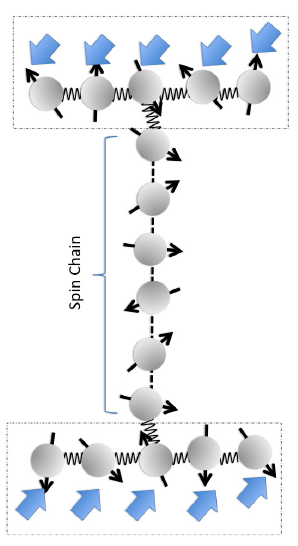
\includegraphics[width=\textwidth]{Images/processor}
		\end{column}
		\uncover<2->{\begin{column}{0.33\textwidth}
			\centering
    		Computers
    		\includegraphics[trim=0 0 0 -40mm, width=\textwidth]{Images/computer}
		\end{column}}
     	\uncover<3->{\begin{column}{0.33\textwidth}
     		\centering
     		Computing
     		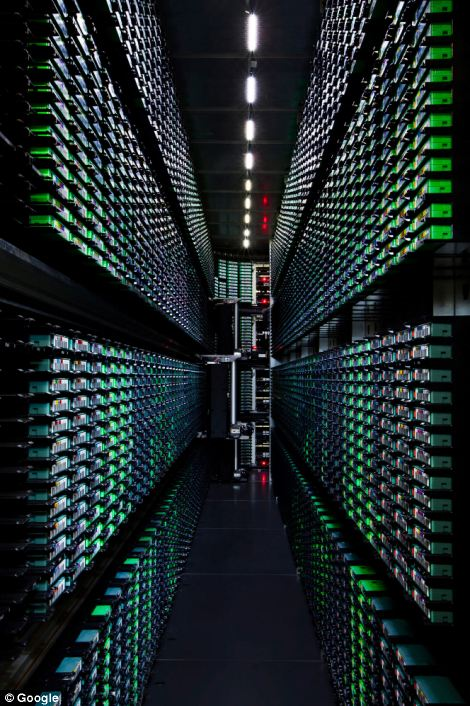
\includegraphics[trim=0 0 0 -20mm, width=\textwidth]{Images/computing}
		\end{column}}
	\end{columns}
\end{frame}

\subsection{Requirements}
\begin{frame}{Requirements}
	\begin{itemize}
		\item Separation of highly controlled regions
		\item Spacers
		\begin{itemize}
			\item (Perfect) state transfer
			\item Fixed interactions
			\item Natural dynamics
			\item Control single qubit at each end only (for now)
		\end{itemize}
	\end{itemize}
	
	$\rightarrow$ Spin networks!
%Registers are highly controlled regions (gates, ...), probably need separation, spacers need to be capable of state transfer -> spins, control free region: permanent, fixed interactions between spins, natural dynamics (initialize, wait, read); For now: only single qubits control at each site, homogenous constant couplings, PST (Explain!), spin networks instead so no transformation is needed.
\end{frame}

\subsection{Model}
\begin{frame}[t]{Model}	
	\begin{exampleblock}{}
	\setlength\abovedisplayskip{-8pt}
	\begin{center}
		\[H_{XX}=\frac{1}{2}J\sum_{i=1}^{N}{\left[\sigma_i^x\sigma_{i+1}^x + \sigma_i^y\sigma_{i+1}^y\right]}\]
	\end{center}
	\end{exampleblock}
	\begin{itemize}
		\item $J\equiv const.$
		\item No z coupling
		\item $\left[H_{XX},\sigma^z_\text{tot}\right] = 0$
		\item Eigenstates: $\ket{\tilde{k}} = \sqrt{\frac{2}{N+1}}\sum_{s=1}^N\sin\left(\frac{\pi ks}{N+1}\right)\ket{s}$
		\item Eigenvalues: $ E_k = 2\cos\left(\frac{\pi k}{N+1}\right)$
	\end{itemize}
%    Show complete Heisenberg model (no local potentials), explain terms, why no z coupling etc., commutes with total z spin, then XY model, what do states look like?
\end{frame}

\subsection{Math setup}
\begin{frame}{Math setup}
	\begin{description}
	\item [Ground state of ferromagnetic spin-$\frac{1}{2}$ chain:] \[ \ket{\uparrow}_1 \otimes \ket{\uparrow}_2 \otimes \dots \otimes \ket{\uparrow}_N = \ket{\uparrow_1\uparrow_2\dots\uparrow_N} := \ket{0} \]
	\item [Excitation operator $\sigma^- = \frac{1}{2}\left(\sigma^x - \text{i}\sigma^y\right)$:] \[ \text{1}_1 \otimes \text{1}_2 \otimes \dots \otimes \text{1}_{s-1} \otimes \sigma^- \otimes \text{1}_{s+1} \otimes \dots \otimes \text{1}_N := \sigma^-_s \]
	\item [Single spin excitation:] \[ \sigma^-_s\ket{0} := \ket{s} \]
	\item [Single spin superposition:] Prepare spin at $s$ as $\alpha\ket{\uparrow}_s + \beta\ket{\downarrow}_s \rightarrow$ \[ \ket{\Psi} := \alpha\ket{0} + \beta\ket{s} \]
	\end{description}
%    Explain numbers as kets, superpositions, graphs, later binary scheme for graphs, adjacency matrices and correspondence to hamiltonian, fidelity.
\end{frame}

\begin{frame}{Perfect state transfer}
%	In general, target state will evolve into a mixed state:\\
	\[ \ket{\Psi_{in}} = \cos{\left(\frac{\Theta}{2}\right)} \ket{0} + e^{\text{i}\Phi}\sin{\left(\frac{\Theta}{2}\right)}\ket{s} \]
	\[ \ket{\Psi_{out}} = \frac{1}{\sqrt{P(t)}}\left( \cos{\left(\frac{\Theta}{2}\right)} \ket{0} + e^{\text{i}\Phi}\sin{\left(\frac{\Theta}{2}\right)}f^N_{r,s}(t)\ket{r} \right) \]
	\[ \rho_{out} = P(t)\ket{\Psi_{out}}\bra{\Psi_{out}} + \left( 1-P(t) \right)\ket{\uparrow}\bra{\uparrow} \]
%	and
%	\[ P(t) = \cos^2{\left(\frac{\Theta}{2}\right)} + \sin^2{\left(\frac{\Theta}{2}\right)}\lvert f^N_{r,s}(t)\rvert^2 \]
	Transition amplitude: $f^N_{r,s}(t) = \bra{r}e^{\text{i}H t}\ket{s}$\\
	\begin{exampleblock}{Fidelity:}
	\setlength\abovedisplayskip{-8pt}
	\begin{center}
		\[ \mathfrak{F}(t) = \frac{1}{4\pi}\int \!\bra{\Psi_{in}}\rho_{out}\ket{\Psi_{in}} \, \mathrm{d}\Omega = \frac{\lvert f^N_{r,s}\rvert\cos{\lambda}}{3} + \frac{\lvert f^N_{r,s}\rvert^2}{6} + \frac{1}{2}\]
% in order to give qualitative statements it suffices to know f^N_r,s
	\end{center}
	\end{exampleblock}
\end{frame}

\begin{frame}[t]{Graphs}
	\begin{exampleblock}{}
	\setlength\abovedisplayskip{-8pt}
	\begin{center}
		$G = (V,E)$
	\end{center}
	\end{exampleblock}
	\begin{itemize}
		\item Edges undirected $\rightarrow E \subseteq \{\{i,j\}\colon i,j \in V\}$
		\item Single edges only $\rightarrow \{i,j\}$ unique
	\end{itemize}   
%	is a subset of the set of all unordered pairs of vertices in $V$.
	Example: $V = \{1,2,3\}, E = \{\{1,2\},\{2,3\}\}$
		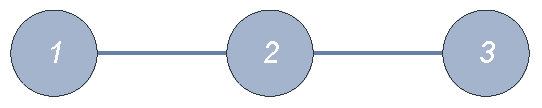
\includegraphics[trim=0 0 0 -5mm, width=\textwidth]{Images/chain3}
\end{frame}

\begin{frame}[t]{Adjacency Matrices}
	\begin{exampleblock}{}
	\setlength\abovedisplayskip{-8pt}
	\begin{center}
		$a_{ij} = \left\{
	\begin{array}{ll}
		1  & \{i,j\} \in E \\
		0  & \text{otherwise}
	\end{array}
\right.$	
	\end{center}
	\end{exampleblock}
	\begin{itemize}
		\item No multi-edges $\rightarrow$ all elements either $0$ or $1$
		\item Unordered Pairs $\rightarrow$ symmetric
		\item Orthogonal basis exists, eigenvalues are roots of $det(A-\lambda \text{1}) = 0$
	\end{itemize}
	\begin{columns}[T]
		\begin{column}{0.5\textwidth}
			\centering
   			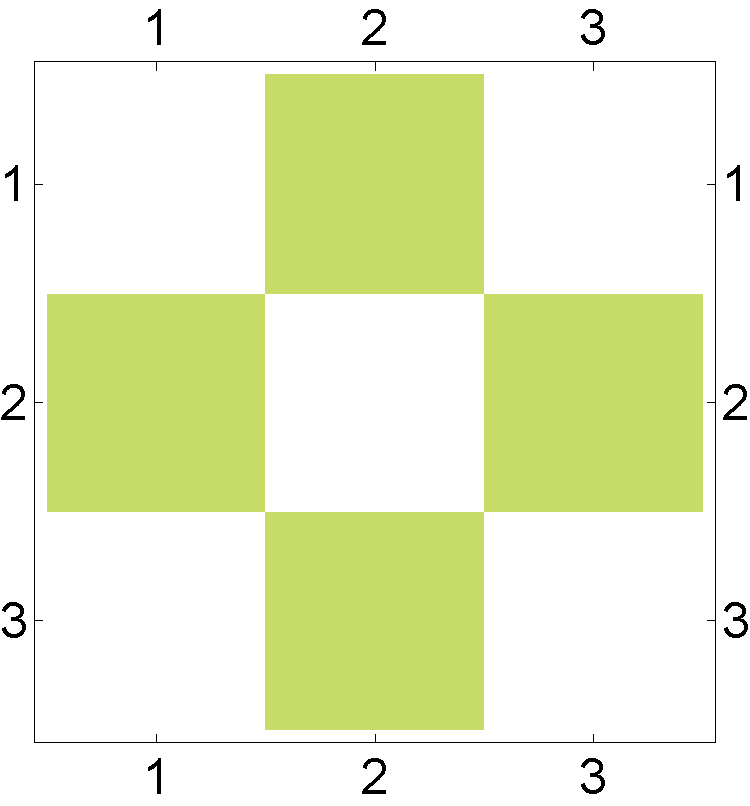
\includegraphics[trim=0 0 0 5mm, width=0.5\textwidth]{Images/adj_chain3}
		\end{column}
		\begin{column}{0.5\textwidth}
			\centering
    		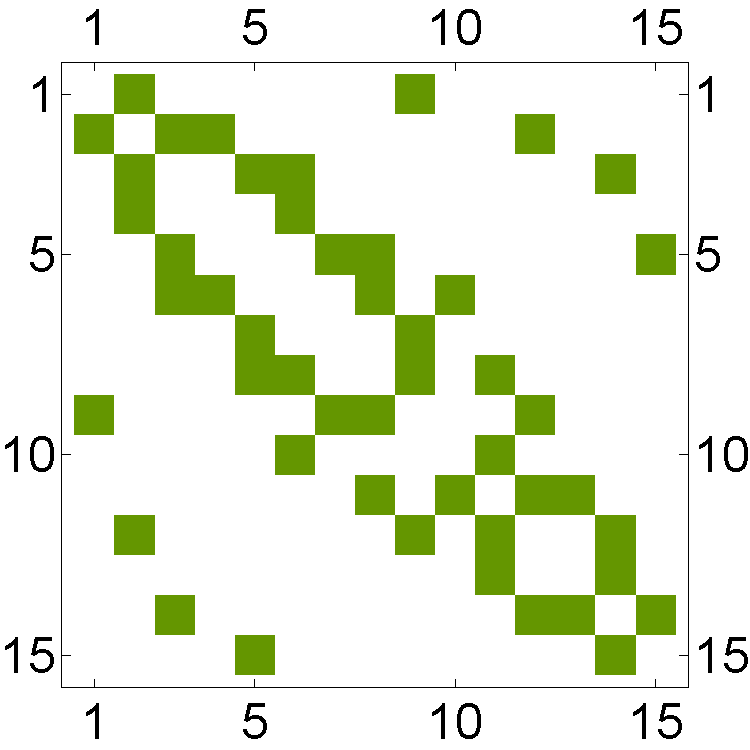
\includegraphics[trim=0 0 0 18mm, width=0.6\textwidth]{Images/adj_ring6_2}
		\end{column}
	\end{columns}
\end{frame}

\begin{frame}{Correspondence to Hamiltonians}
	\begin{columns}[T]
		\begin{column}{0.33\textwidth}
			\centering
   			6-qubit ring
   			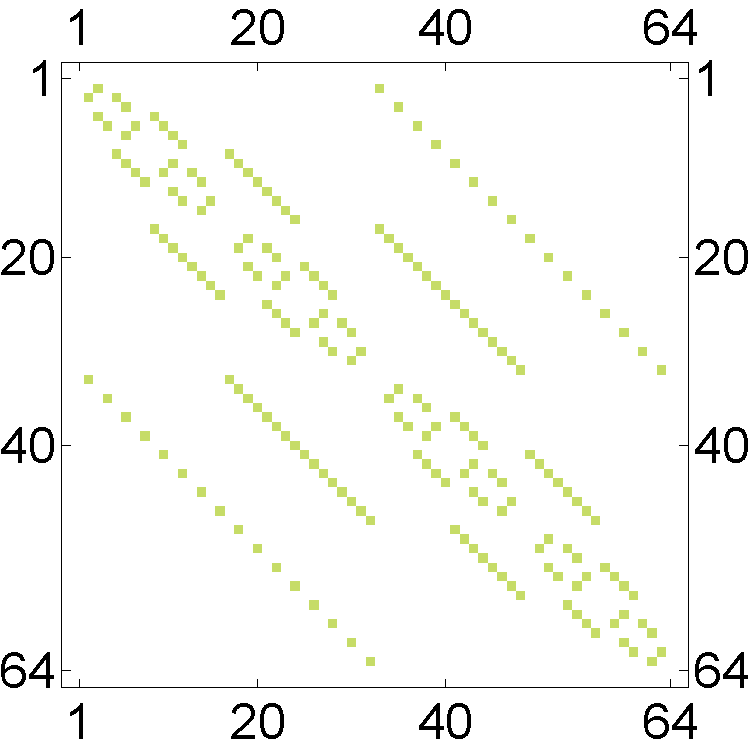
\includegraphics[width=\textwidth]{Images/ring6_hamilton}
		\end{column}
		\uncover<2->{\begin{column}{0.33\textwidth}
			\centering
    		Graph
    		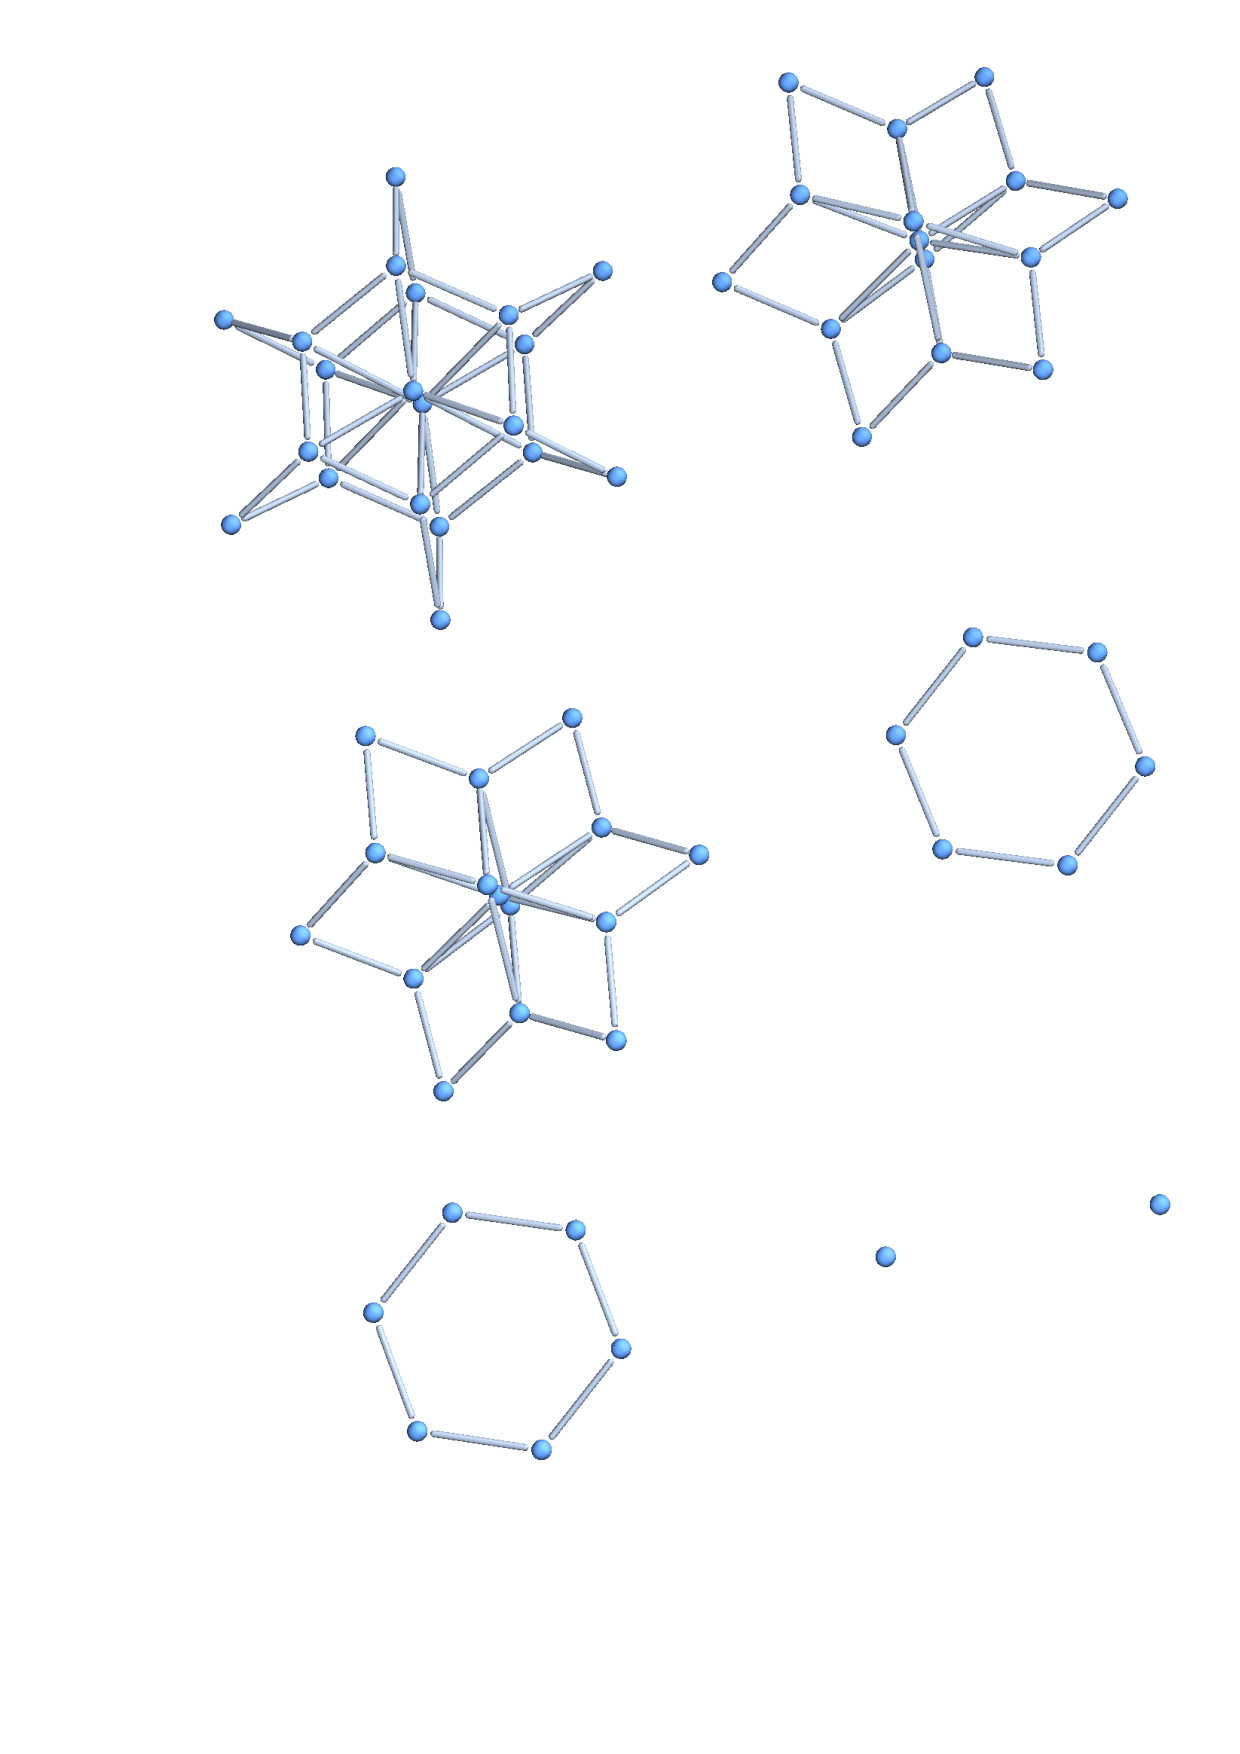
\includegraphics[trim=0 0 0 0mm, width=\textwidth]{Images/ring6_hamilton_graph3d}
		\end{column}}
     	\uncover<3->{\begin{column}{0.33\textwidth}
     		\centering
     		Single spin subspace
     		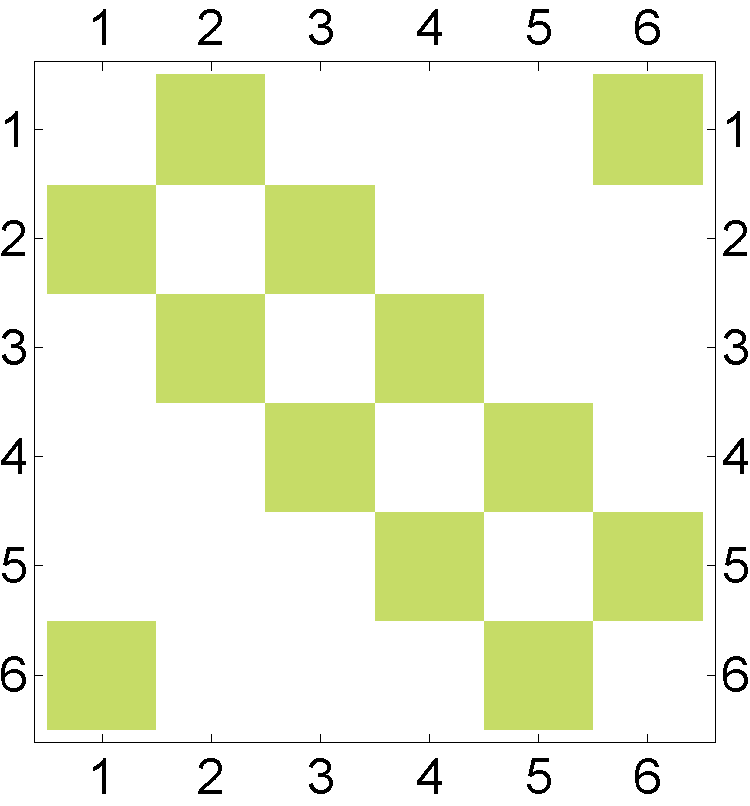
\includegraphics[trim=0 0 0 0mm, width=\textwidth]{Images/adj_ring6_1}\\
     		\uncover<4->{This is the adjacency matrix for the 6-qubit ring!}
		\end{column}}
	\end{columns}
\end{frame}

\begin{frame}{How to identify subspaces}
	\begin{columns}[T]
		\begin{column}{0.5\textwidth}
			\centering
   			Recipe:
   			\begin{itemize}
   				\item Matrix labels $-1$
   				\item Convert labels to binary
   				\item Identify rows and columns with equal number of $1$s (e.g. 1)
   				\item Strip off all other rows and columns
   				\item Compile matrix from rows and columns left
   				\item ${N \choose s}$ vertices (states) in graph
   			\end{itemize}
   		\end{column}
		\begin{column}{0.5\textwidth}
			\centering
    		Graph
    		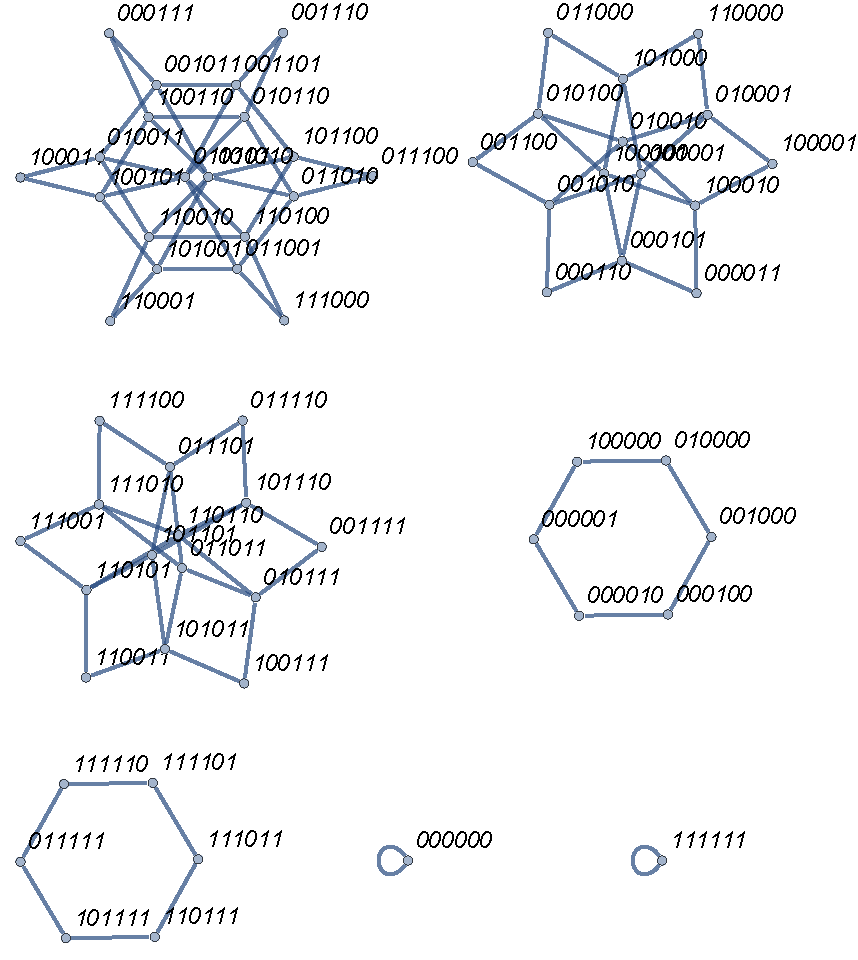
\includegraphics[trim=0 0 0 0mm, width=\textwidth]{Images/ring6_hamilton_graph3d_alt}
		\end{column}
	\end{columns}
\end{frame}

\begin{frame}[t]{Cartesian Product of Graphs}
	\begin{exampleblock}{}
	\setlength\abovedisplayskip{-8pt}
	\begin{center}
		$G \times H = (V_{G\times H},E_{G\times H})$
	\end{center}
	\end{exampleblock}
	\begin{itemize}
		\item $V_{G\times H} = V(G) \times V(H)$
		\item $\{(u,u'),(v,v')\} \in E_{G\times H}$ if 
		\begin{itemize}
			\item $u = v$ and $\{u',v'\} \in E_H$ or
			\item $u' = v'$ and $\{u,v\} \in E_G$
		\end{itemize}
	\end{itemize}
	\begin{exampleblock}{}
	\setlength\abovedisplayskip{-8pt}
	\begin{center}
		$A_{G\times H} = A_G \otimes \text{1}_{\left|V_H\right|} + \text{1}_{\left|V_G\right|} \otimes A_H$
	\end{center}
	\end{exampleblock}
\end{frame}

\begin{frame}{Examples of Product Graphs}
	\begin{columns}[T]
		\begin{column}{0.33\textwidth}
			\centering
   			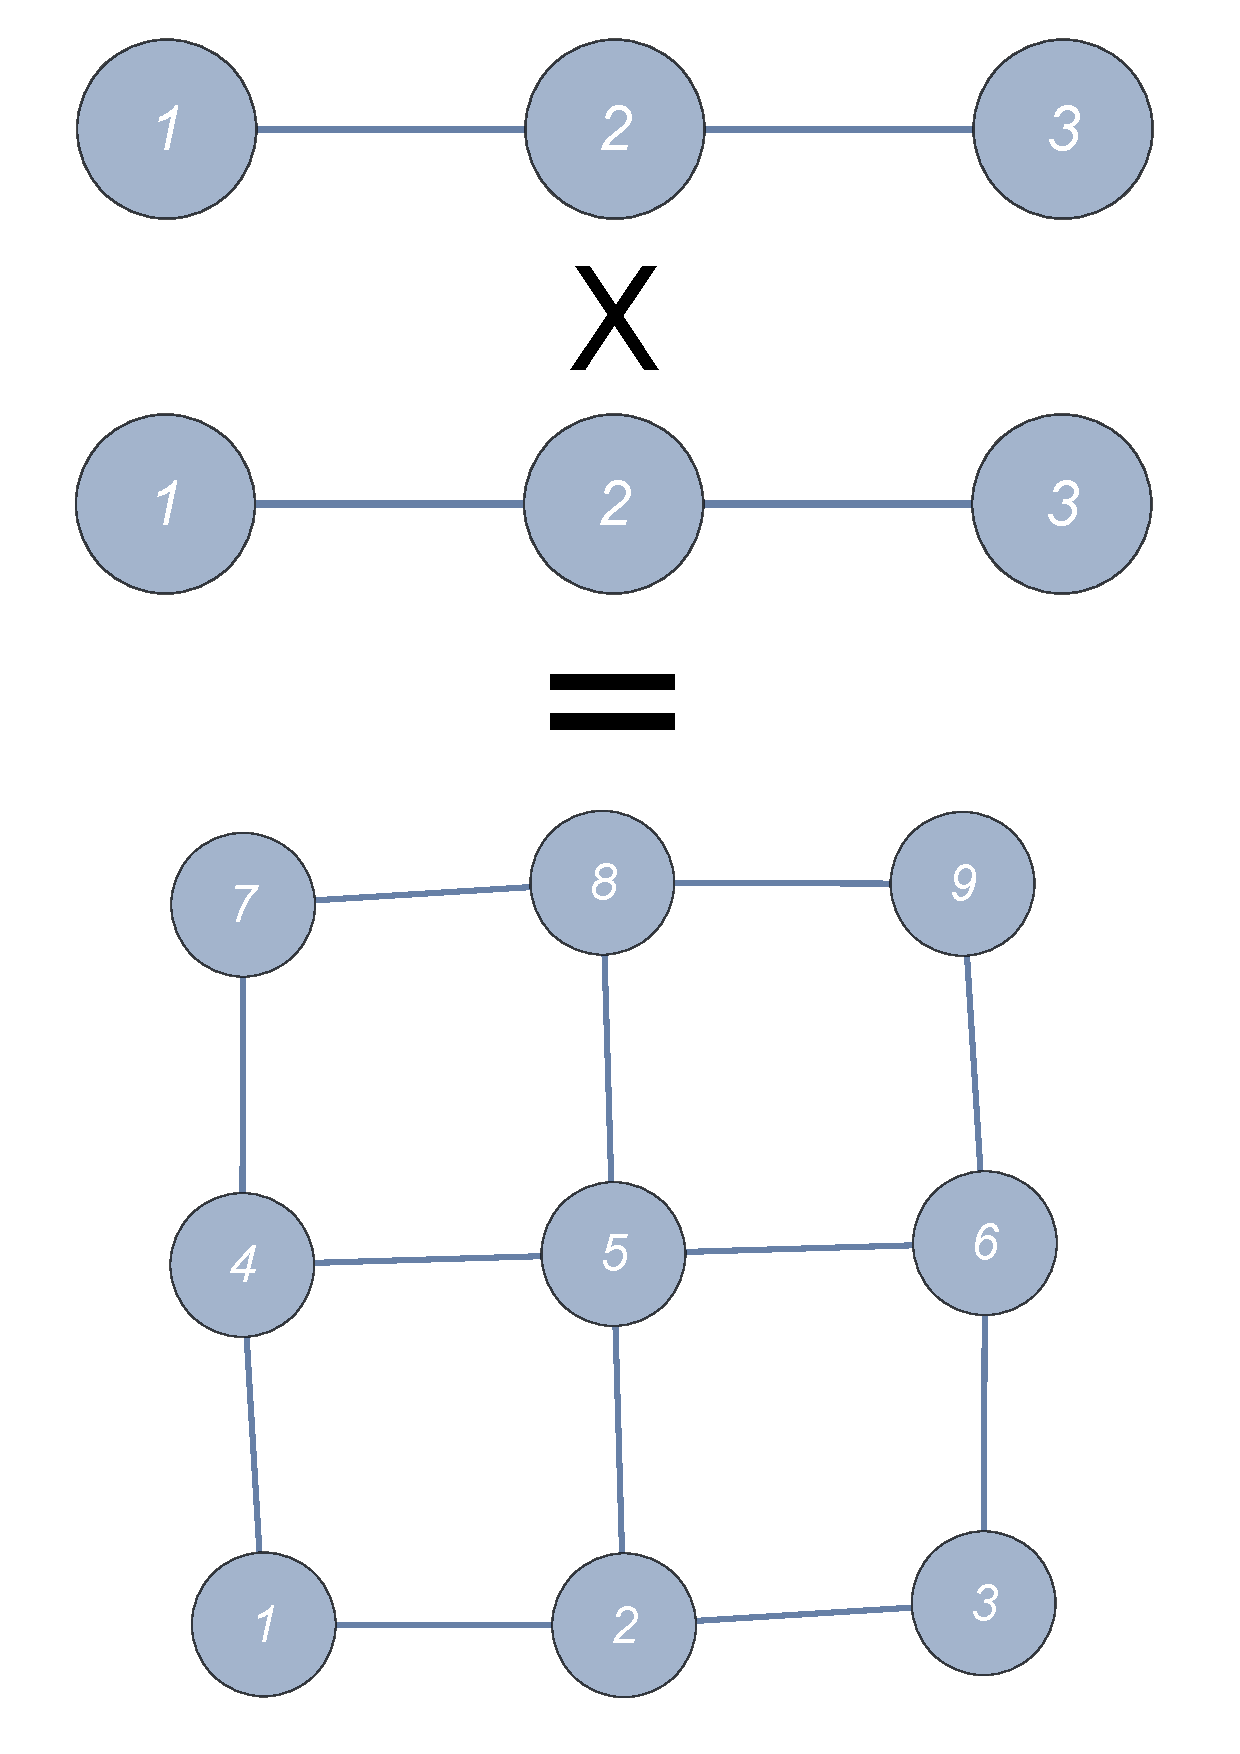
\includegraphics[width=\textwidth]{Images/graphprod_chain3_square}
		\end{column}
		\uncover<2->{\begin{column}{0.33\textwidth}
			\centering
    		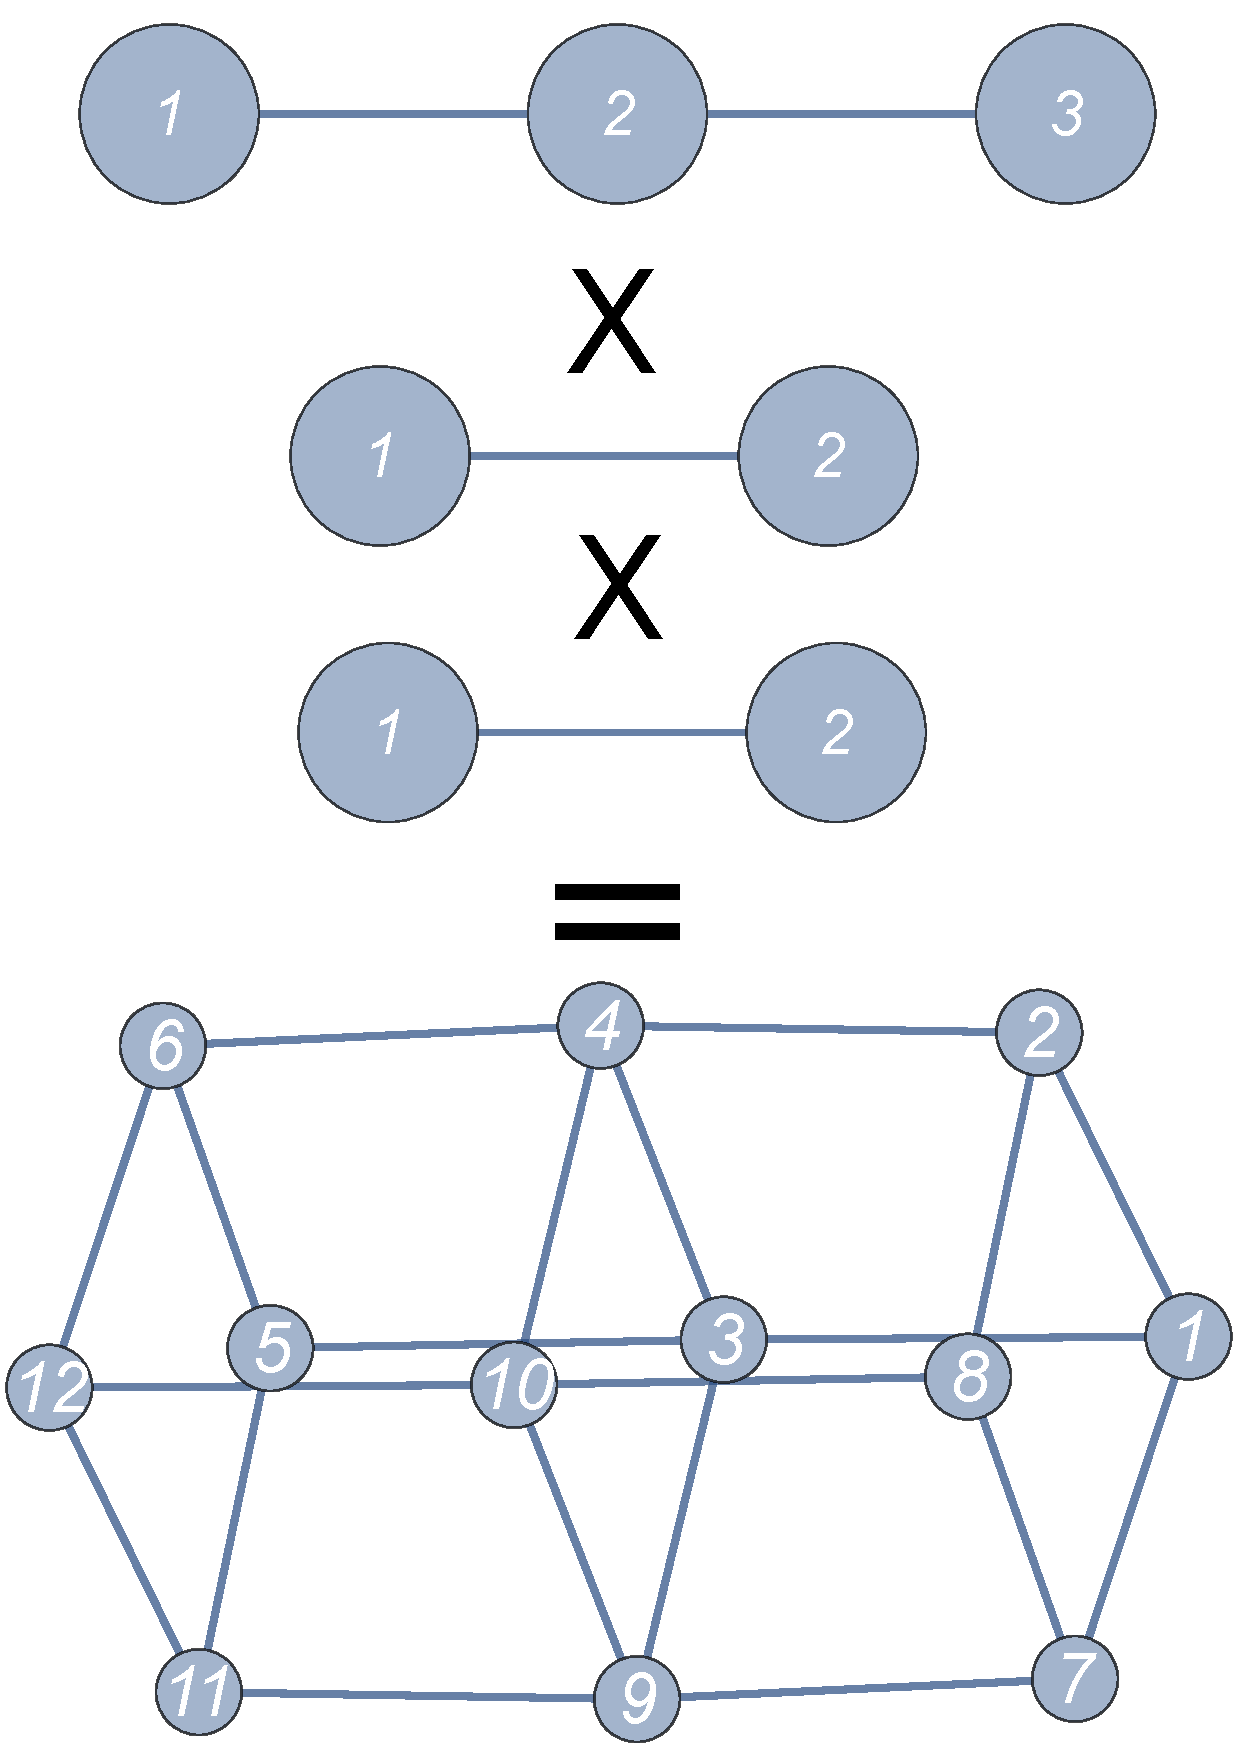
\includegraphics[trim=0 0 0 -10mm, width=\textwidth]{Images/graphprod_chain3_chain2_square}
		\end{column}}
     	\uncover<3->{\begin{column}{0.33\textwidth}
     		\centering
     		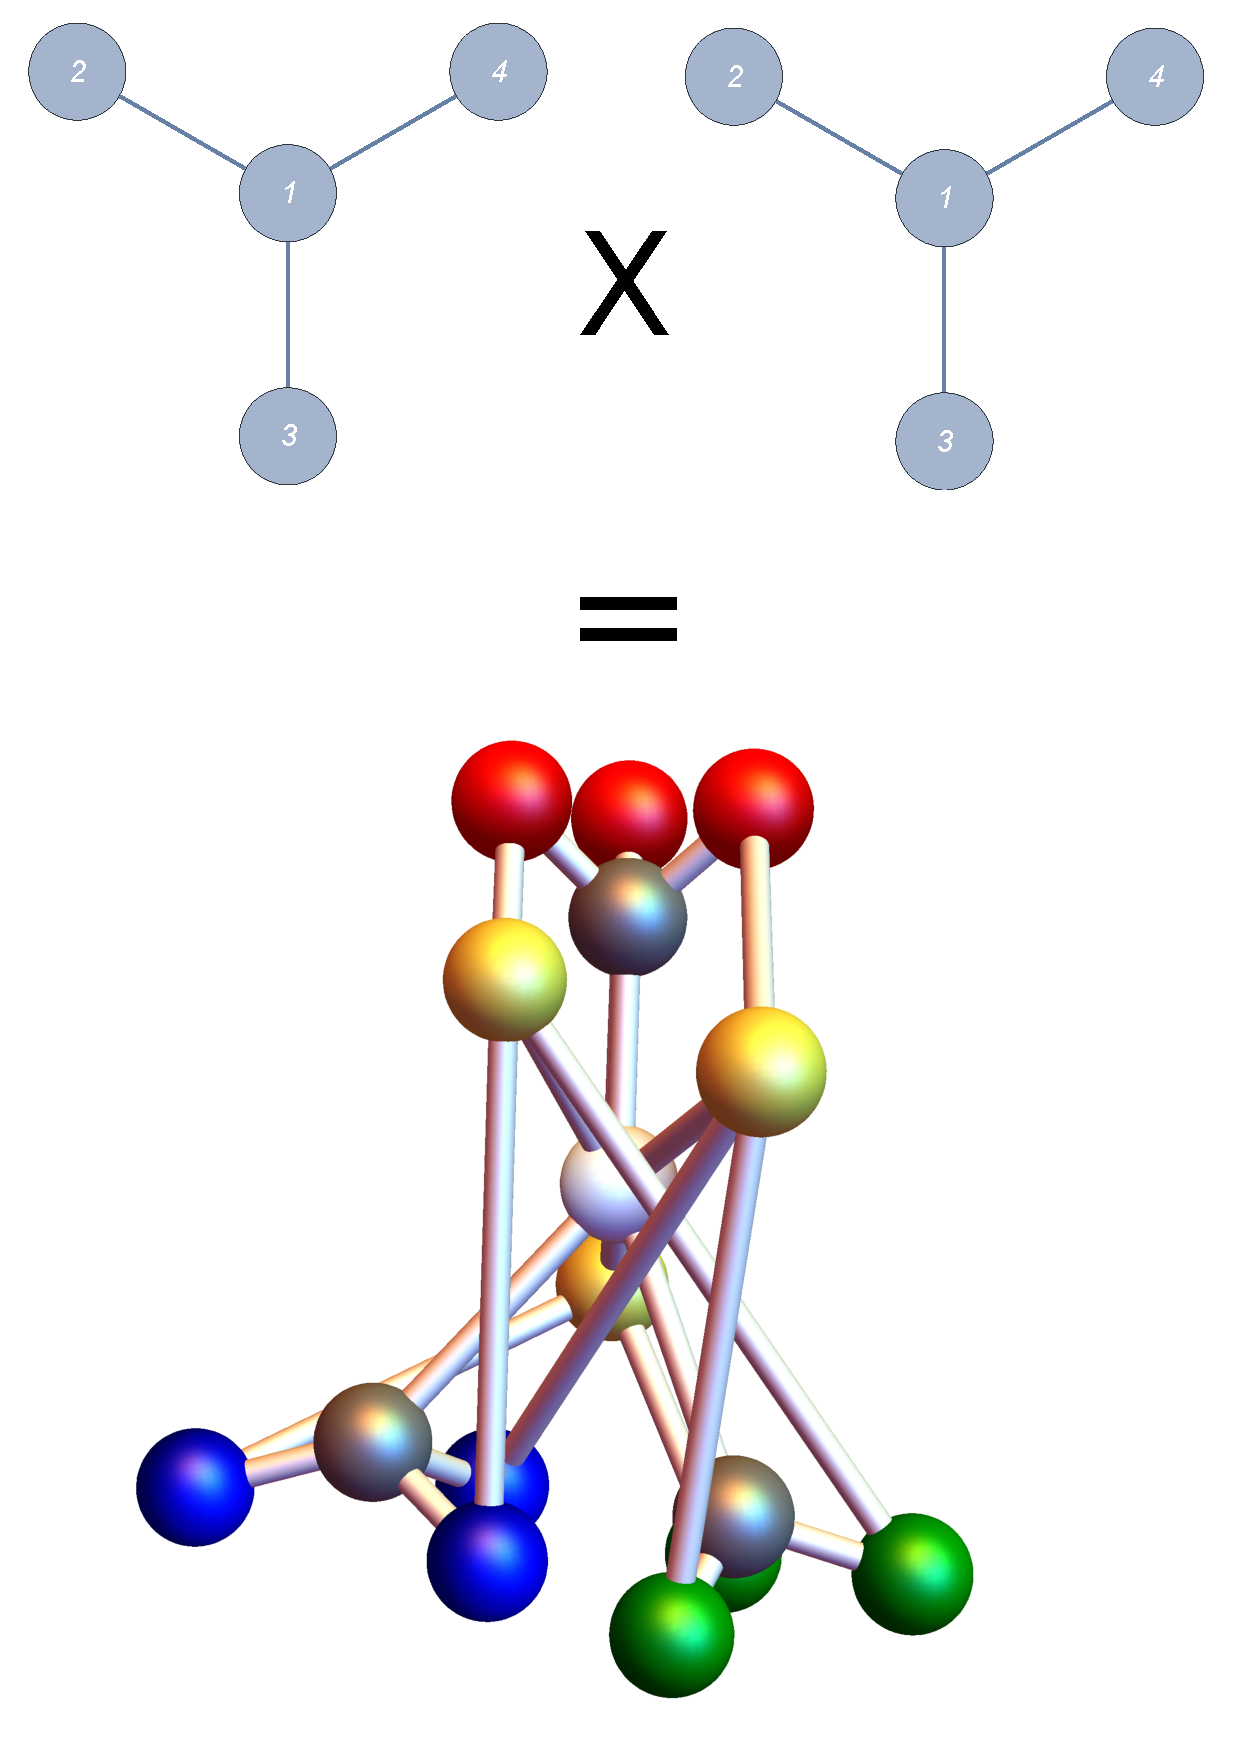
\includegraphics[trim=30mm 0 0 0, width=\textwidth]{Images/graphprod_switch_square}
		\end{column}}
	\end{columns}
\end{frame}

\begin{frame}{Fidelity on Product Graphs}
	\begin{align*}
		f^{\left|V_{G\times H}\right|}_{(r,r'),(s,s')}(t) &= \left( \bra{r} \otimes \bra{r'} \right)e^{-\text{i}A_{G\times H}t} \left( \ket{s} \otimes \ket{s'} \right) \\
		&= \left( \bra{r} \otimes \bra{r'} \right)e^{-\text{i}(A_G \otimes \text{1}_{\left|V_H\right|})t} e^{-\text{i}(\text{1}_{\left|V_G\right|} \otimes A_H)t} \left( \ket{s} \otimes \ket{s'} \right) \\
		&= \sum_{k=1}^{K}\left[ \left( \bra{r} \otimes \bra{r'} \right) \ket{g'_k}\bra{g'_k}e^{-\text{i}G_k{}'t} \ket{h_k'}\bra{h_k'}e^{-\text{i}H_k{}'t} \left( \ket{s} \otimes \ket{s'} \right) \right]
	\end{align*}
	%\begin{align*}
		%f^{G\times H}_{N\times N'}(t) &= \left( \bra{N} \otimes \bra{N'} \right)e^{-\text{i}A_{G\times H}t} \left( \ket{1} \otimes \ket{1'} \right) \\
		%&= \left( \bra{N} \otimes \bra{N'} \right)e^{-\text{i}(A_G \otimes \text{1}_{\left|V_H\right|})t} e^{-\text{i}(\text{1}_{\left|V_G\right|} \otimes A_H)t} \left( \ket{1} \otimes \ket{1'} \right) \\
		%&= \sum_{k=1}^{K}\left[ \left( \bra{N} \otimes \bra{N'} \right) \ket{g'_k}\bra{g'_k}e^{-\text{i}G_k{}'t} \ket{h_k'}\bra{h_k'}e^{-\text{i}H_k{}'t} \left( \ket{1} \otimes \ket{1'} \right) \right]
	%\end{align*}
	\begin{itemize}
		\item $K = \left|V_{G\times H}\right|$, $L = \left|V_G\right|$, $M = \left|V_H\right| \rightarrow K = L\cdot M$
		\item $\bra{g'_k} = \bra{g_l} \otimes \bra{e_m}$, $\bra{h'_k} = \bra{e_l} \otimes \bra{h_m}$ etc.
		\item $G_k{}' = G_l\cdot E_m$, $H_k{}' = E_l\cdot H_m$
		\item $(A\otimes B)(C\otimes D) = (AC)\otimes (BD)$
	\end{itemize}
	\begin{align*}
		f^{\left|V_{G\times H}\right|}_{(r,r'),(s,s')}(t) &= \sum_{l=1}^L\left[ \Braket{r|g_l}\Braket{g_l|s}e^{-\text{i}G_l t} \right] \sum_{m=1}^M\left[ \Braket{r'|h_m}\Braket{h_m|s'}e^{-\text{i}H_mt} \right] \\
		&= \Braket{r|e^{-\text{i}A_G t}|s}\Braket{r'|e^{-\text{i}A_H t}|s'}
	\end{align*}
\end{frame}

\begin{frame}[t]{Fidelity on Product Graphs}
	\begin{exampleblock}{}
	\setlength\abovedisplayskip{-8pt}
	\begin{center}
		$ f^{\left|V_{G\times H}\right|}_{(r,r'),(s,s')}(t) = f^{\left|V_G\right|}_{r,s}(t)\cdot f^{\left|V_H\right|}_{r',s'}(t) $
	\end{center}
	\end{exampleblock}
	\begin{align*}
		f^{\left|V_G\right|}_{r,s}(t) &= 1 \text{ for } t = \tau_G \\ 
		f^{\left|V_H\right|}_{r',s'}(t) &= 1 \text{ for } t = \tau_H \\ 
		f^{\left|V_{G\times H}\right|}_{(r,r'),(s,s')}(t) &= 1 \text{ for } t = \tau_{G\times H}
	\end{align*}
	\begin{exampleblock}{}
	\setlength\abovedisplayskip{-8pt}
	\begin{center}
		$ \text{iff }\frac{t_G}{t_H} \in \mathbb{Q}$ %\rightarrow t_{G\times H} = LCM(t_G,t_H) $
	\end{center}
	\end{exampleblock}
\end{frame}

\section{Examples}
\subsection{Spin Chains}
\begin{frame}[t]{Spin Chains}
	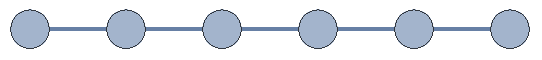
\includegraphics[trim=0 0 0 0, width=\textwidth]{Images/chain6_nolabels}\\
	\[f_{N,1}^N(t) = \frac{2}{N+1}\sum_{s}^N\sin\left(\frac{\pi s}{N+1}\right)\sin\left(\frac{\pi sN}{N+1}\right)e^{-\text{i}E_s t} \]
	\begin{itemize}
		\item $N=2$: \,\,\,\,$f_{2,1}^2(t) = -\text{i}\sin(t)$ \,\,\,\,\,\,\,\,\,\,\,\,\,\,\,\,\,with $\tau_2 = \pi/2$
		\item $N=3$: \,\,\,\,$f_{3,1}^3(t) = -\left[\sin(t/\sqrt{2})\right]^2$ with $\tau_3 = \pi/\sqrt{2}$
		\item $N \geq 4$: \,\,\,\,$f_{N,1}^N(t) \neq 1$\,\,\, $\forall$\,\,$t$
	\end{itemize}
	\begin{columns}[T]
		\begin{column}{0.5\textwidth}
			\centering
			\begin{exampleblock}{}
			\setlength\abovedisplayskip{-8pt}
			\begin{center}
		Proof shows that $f_{N,1}^N(t) = 1$ implies $\frac{\cos\left(\frac{2\pi}{N+1}\right)}{\cos\left(\frac{\pi}{N+1}\right)} \in \mathbb{Q}$
			\end{center}
			\end{exampleblock}
		\end{column}
		\begin{column}{0.5\textwidth}
			\centering
        $H = \begin{pmatrix}
			0 & 1 & 0 & 0 & 0 \\
			1 & 0 & 1 & 0 & 0 \\
			0 & 1 & 0 & ... & 0 \\
			0 & 0 & ... & 0 & 1 \\
			0 & 0 & 0 & 1 & 0 
		\end{pmatrix}$
		\end{column}
	\end{columns}
%    PST, max 3, sketch of proof, fidelity
\end{frame}

\subsection{Spin Networks}
\begin{frame}[t]{Spin Networks}
	\begin{columns}[T]
		\begin{column}{0.33\textwidth}
			\centering
   			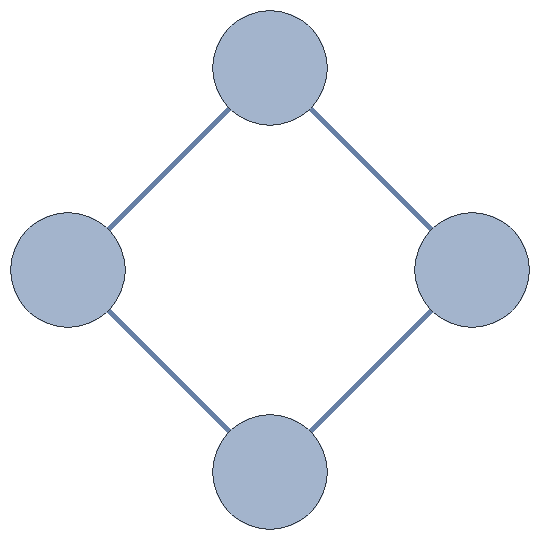
\includegraphics[width=\textwidth]{Images/ring4_nolabels}
		\end{column}
		\begin{column}{0.33\textwidth}
			\centering
    		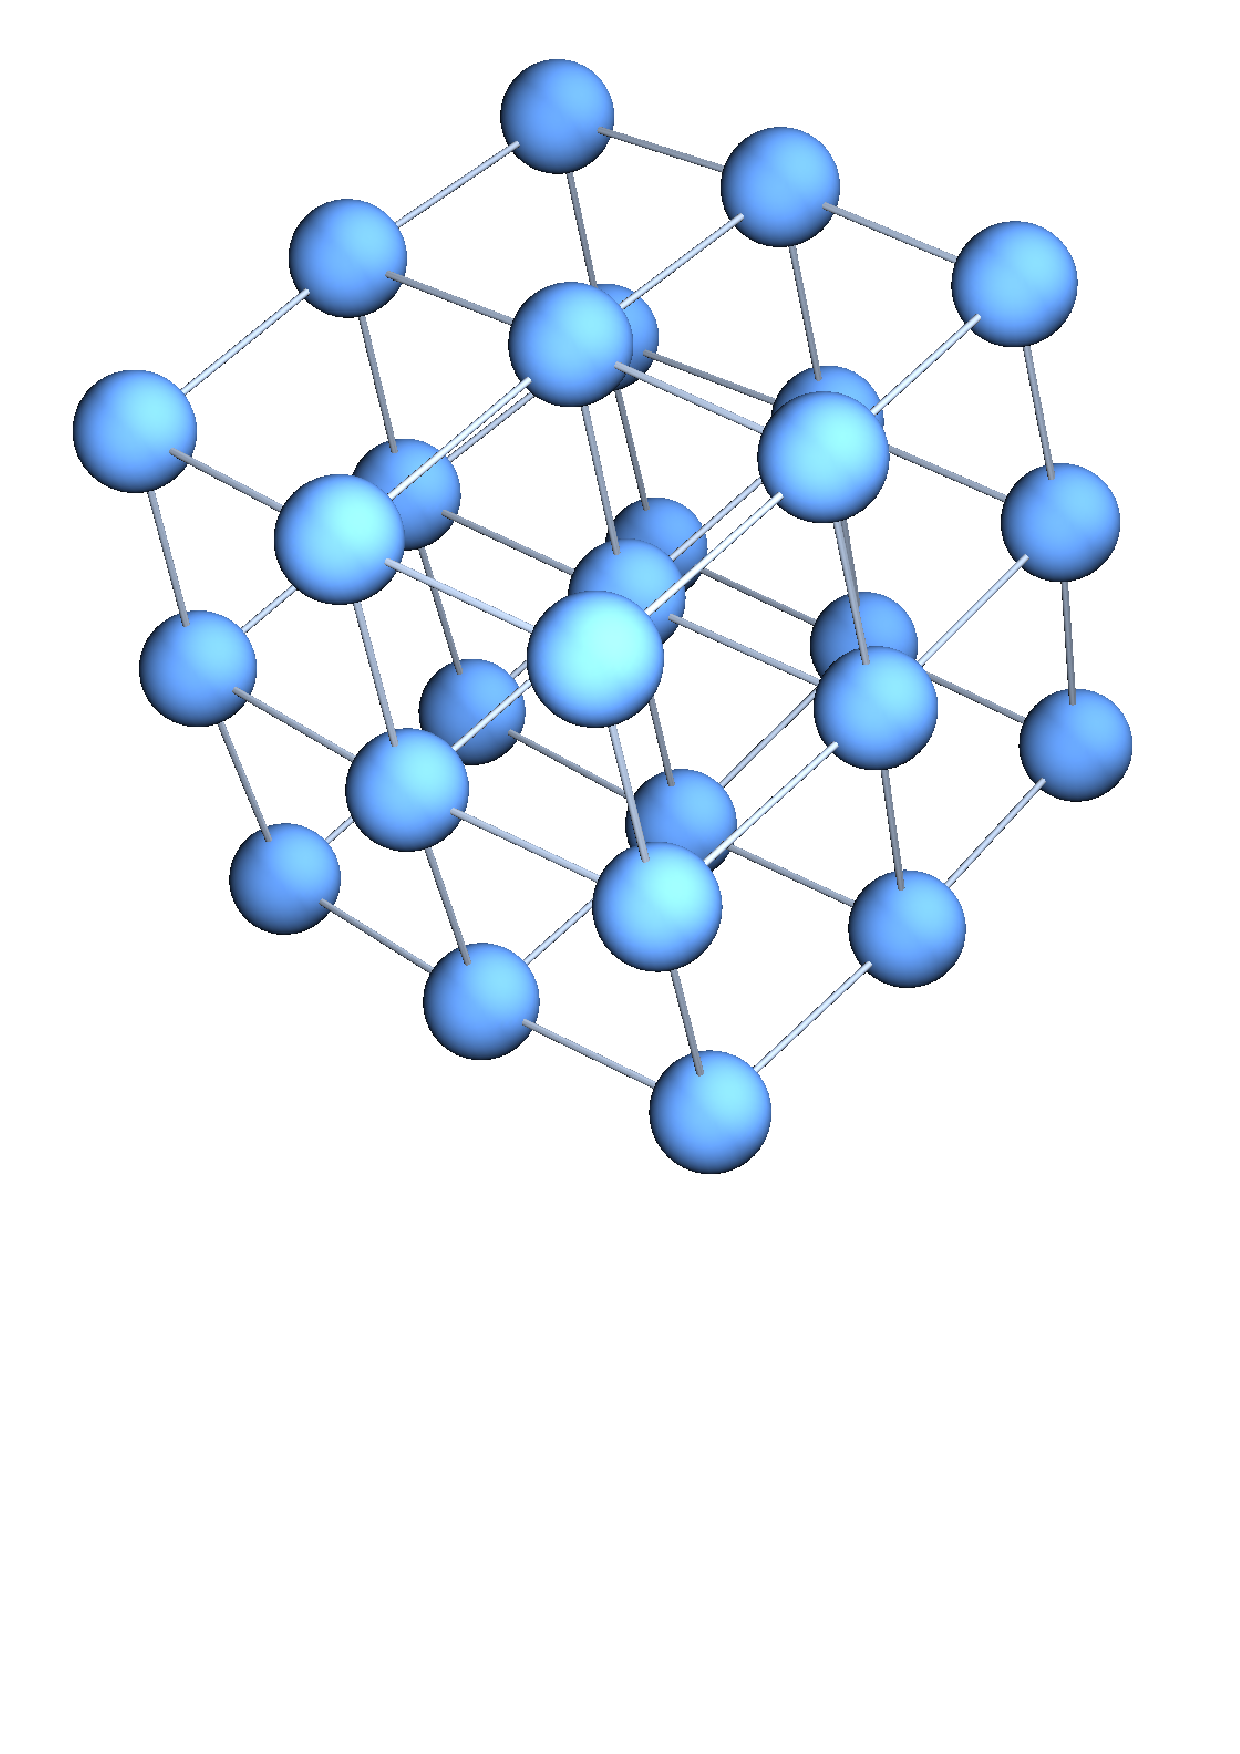
\includegraphics[trim=0 0 0 -10mm, width=\textwidth]{Images/chain3_cubic}\\
    		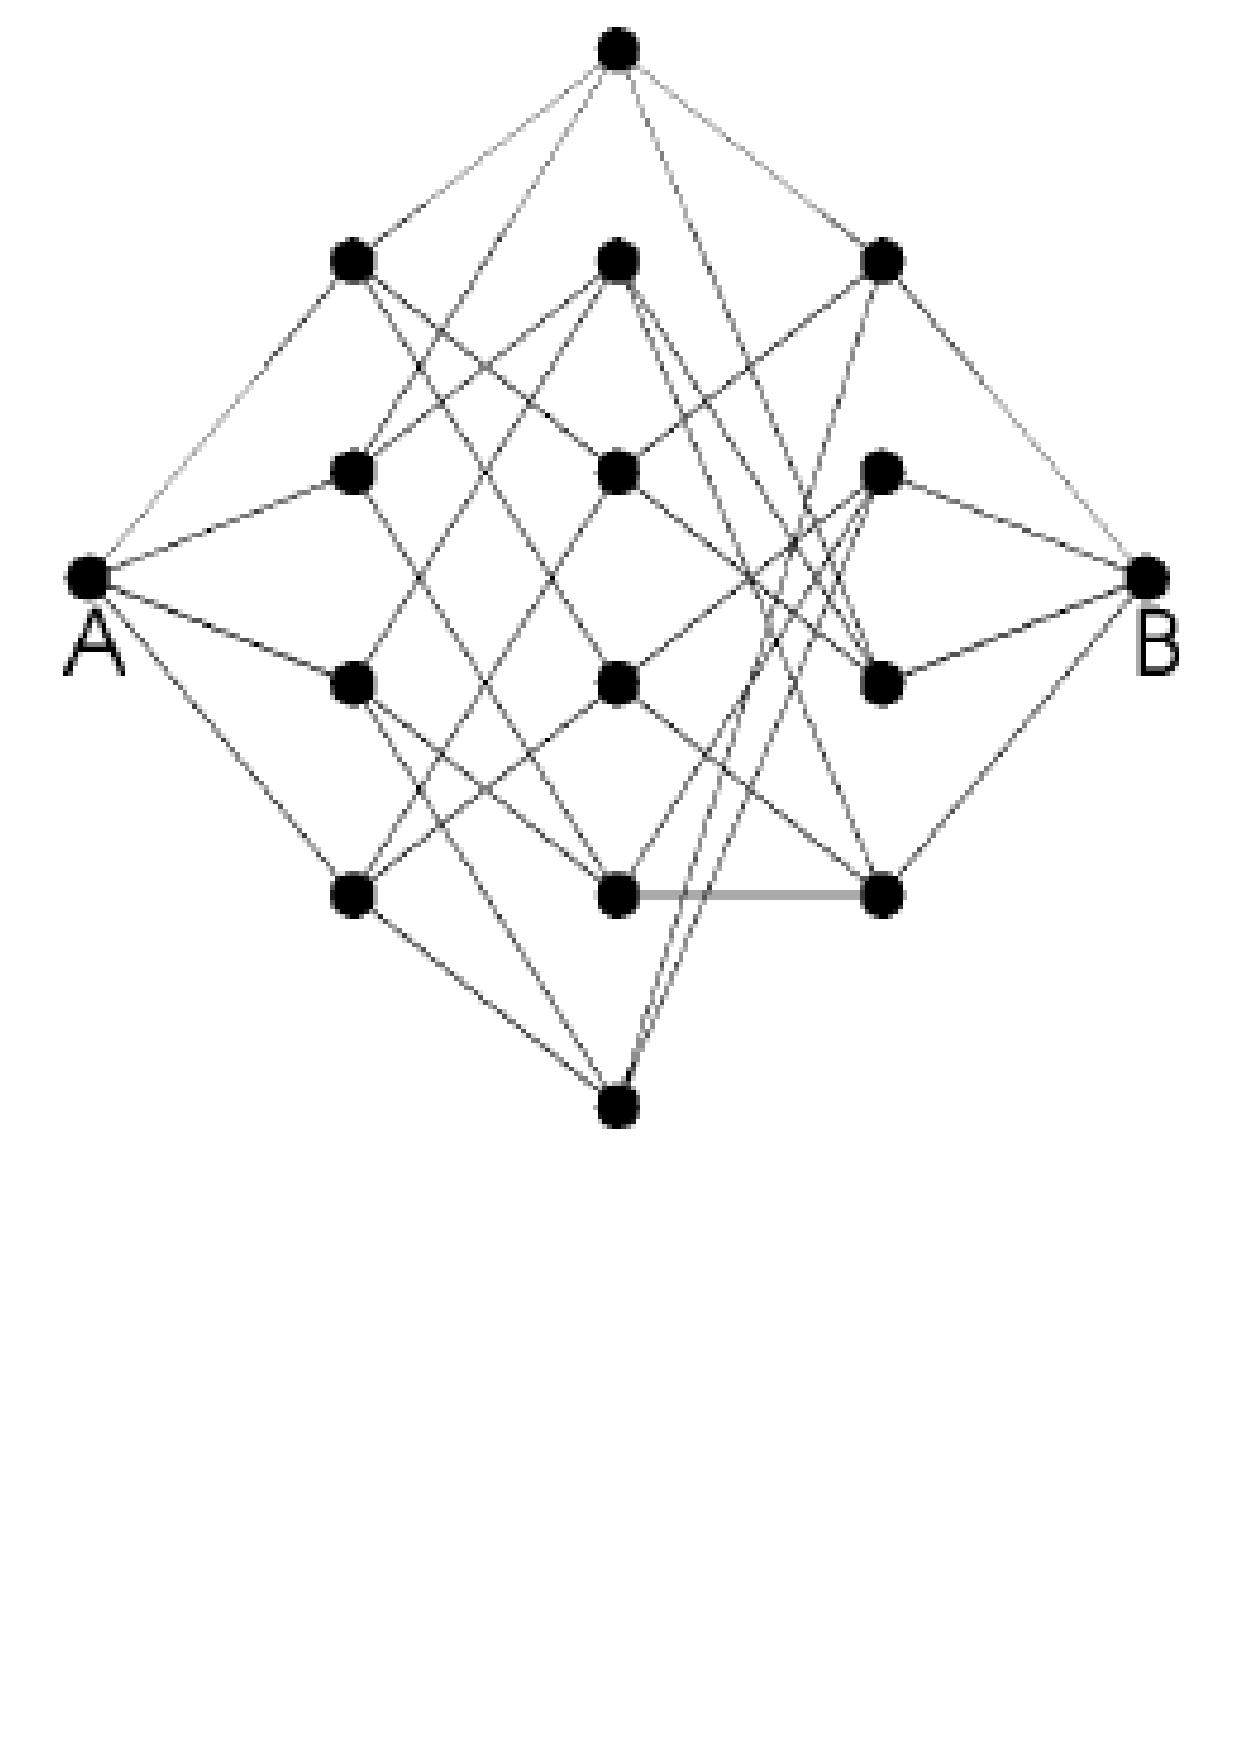
\includegraphics[trim=0 0 0 70mm, width=\textwidth]{Images/chain3_cubic_flattened}
		\end{column}
     	\begin{column}{0.33\textwidth}
     		\centering
     		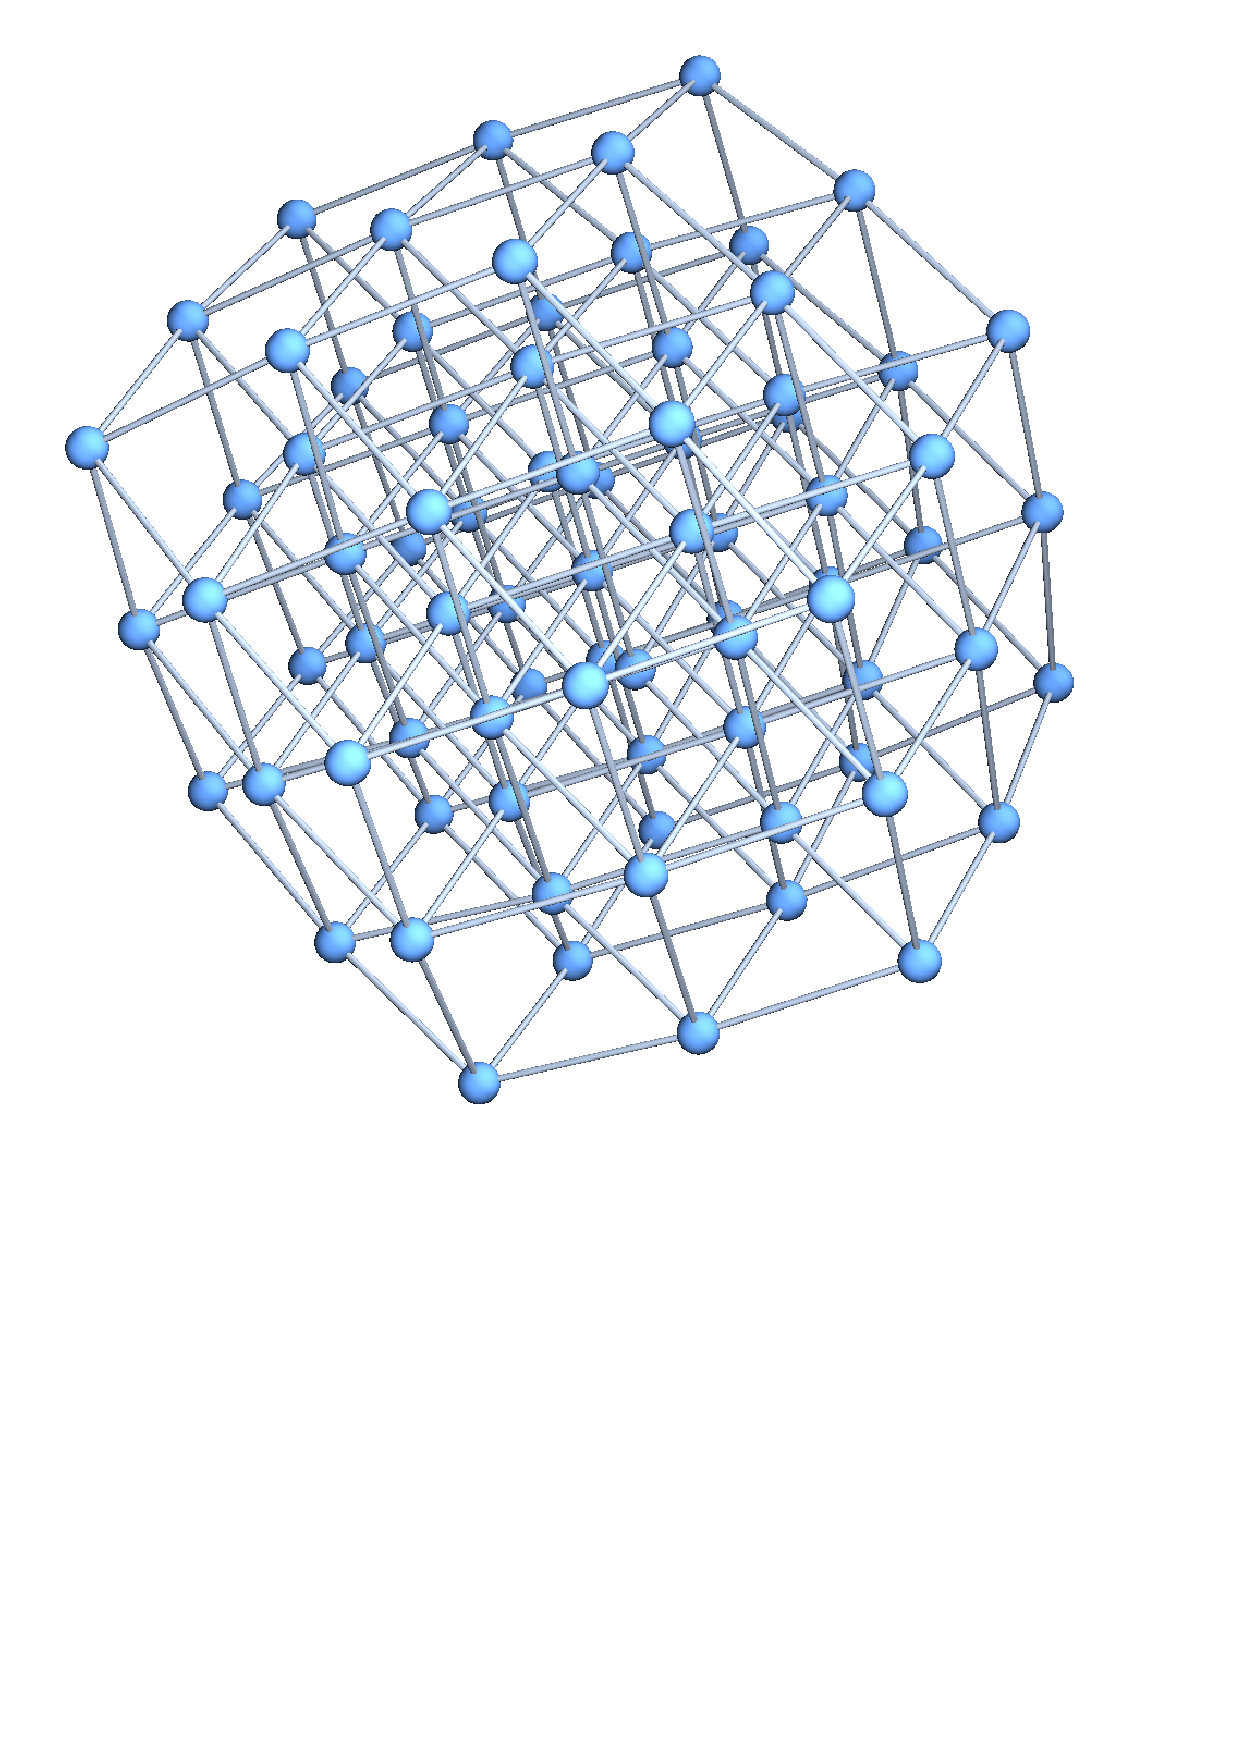
\includegraphics[trim=30mm 0 0 0, width=\textwidth]{Images/chain3_hypercube}
		\end{column}
	\end{columns}
%    Spin chains too short -> more complex networks, explain kronecker product of graphs, sketch proof for fidelity decomposition, hypercubes, flattened versions.
\end{frame}

\subsection{Spin Switch}
\begin{frame}[t]{Spin Switch}
	\begin{exampleblock}{}
	\setlength\abovedisplayskip{-8pt}
	\begin{center}
		\[ H = J\sum_{i=1}^{N-1}\left[\sigma_0^x\sigma_i^x + \sigma_0^y\sigma_i^y\right] + \sum_{i=0}^{N-1}h_i\sigma_i^z \]
	\end{center}
	\end{exampleblock}
	\begin{columns}[T]
		\begin{column}{0.5\textwidth}
			\centering
   			\begin{itemize}
				\item Introduce local potentials
				\item Slight variations only
				\item Diagonal entries 
				\item E.g. magnetic offset field
			\end{itemize}
		\end{column}
		\begin{column}{0.5\textwidth}
			\centering
    		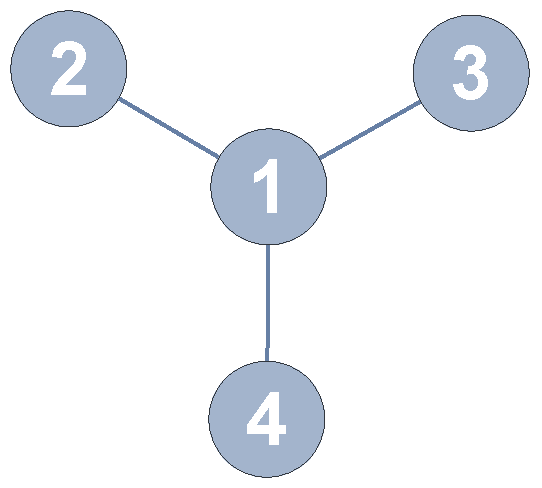
\includegraphics[trim=0mm 0 0 0mm, width=0.8\textwidth]{Images/switch_labeled}
		\end{column}
	\end{columns}
%    Pic of Switch, Variety low, introduce local potentials, only affect diagonal entries, add loops to vertices (left out for clarity), realized as magnetic fields etc.
\end{frame}

\begin{frame}{Spin Switch}
	\begin{columns}[T]
		\begin{column}{0.6\textwidth}
   			\centering
   			\begin{itemize}
   				\item Start: $\ket{\Psi_1} = \alpha \ket{0} + \beta \ket{2}$
   				\item Target: $\ket{\Psi_2} = \alpha \ket{0} + \beta \ket{3}$
   				\item $\braket{3|U(\tau)|2} = \braket{2|U(\tau)|3} \mbeq 1$
   				\item Set $h_2 = h_3$, since $\left[H,P_{23}\right]=0$ 
   				%\[U(\tau)=\sum_{k=0}^3\ket{e_k}\bra{e_k}e^{-\text{i}E_k\tau}\]
   			\end{itemize}
		\end{column}
		\begin{column}{0.4\textwidth}
			\centering
    		$H = \begin{pmatrix}
			h_1 & 1 & 1 & 1 \\
			1 & h_2 & 0 & 0 \\
			1 & 0 & h_3 & 0 \\
			1 & 0 & 0 & h_4
\end{pmatrix}$
		\end{column}
	\end{columns}
	\[\sum_{k=1}^4\bra{2}(P_{23}\ket{e_k})\braket{e_k|2}e^{-\text{i}E_k\tau} \mbeq 1\]\\
   			Choose $E_k$ so they eliminate the phase introduced by $P_{23}$: $E_k \in \{0,h_2,\pm\eta h_2\}$, $\eta$ even.\\
   			Compare $\det(H-\lambda\text{1}_4) = 0$ and $\det(\text{diag}(0,h_2,\pm\eta h_2)-\lambda\text{1}_4) = 0$\\
   			Real roots of the resulting polynomial are solutions for $h_2$, $\tau = \frac{\pi}{h_2}$.
%    sketch calculation, more arms handled by renormalization, fidelities
\end{frame}

\begin{frame}{Spin Switch with more Arms}
			\begin{itemize}
			\item Impose further symmetry condition: $\lambda_4 = \lambda_5 = \dots = \lambda_N$
			\item Renormalize $\ket{4}_{new}=(\ket{4}_{old} + \ket{5} + \dots + \ket{N})/\sqrt{M}$, $M=N-3$
			\end{itemize}
	\begin{columns}
		\begin{column}{0.5\textwidth}
   			\centering
   			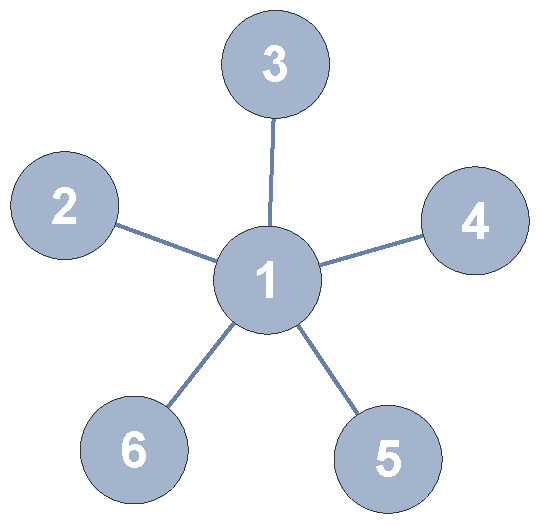
\includegraphics[trim=0mm 0 0 0mm, width=1.2\textwidth]{Images/switch5_labeled}
		\end{column}
		\begin{column}{0.5\textwidth}
			\centering
    		$\tilde{H} = \begin{pmatrix}
			h_1 & 1 & 1 & \sqrt{M} \\
			1 & h_2 & 0 & 0 \\
			1 & 0 & h_3 & 0 \\
			\sqrt{M} & 0 & 0 & h_4
\end{pmatrix}$
		\end{column}
	\end{columns}
%    sketch calculation, more arms handled by renormalization, fidelities
\end{frame}

\begin{frame}[t]{Fidelity}
	\centering
	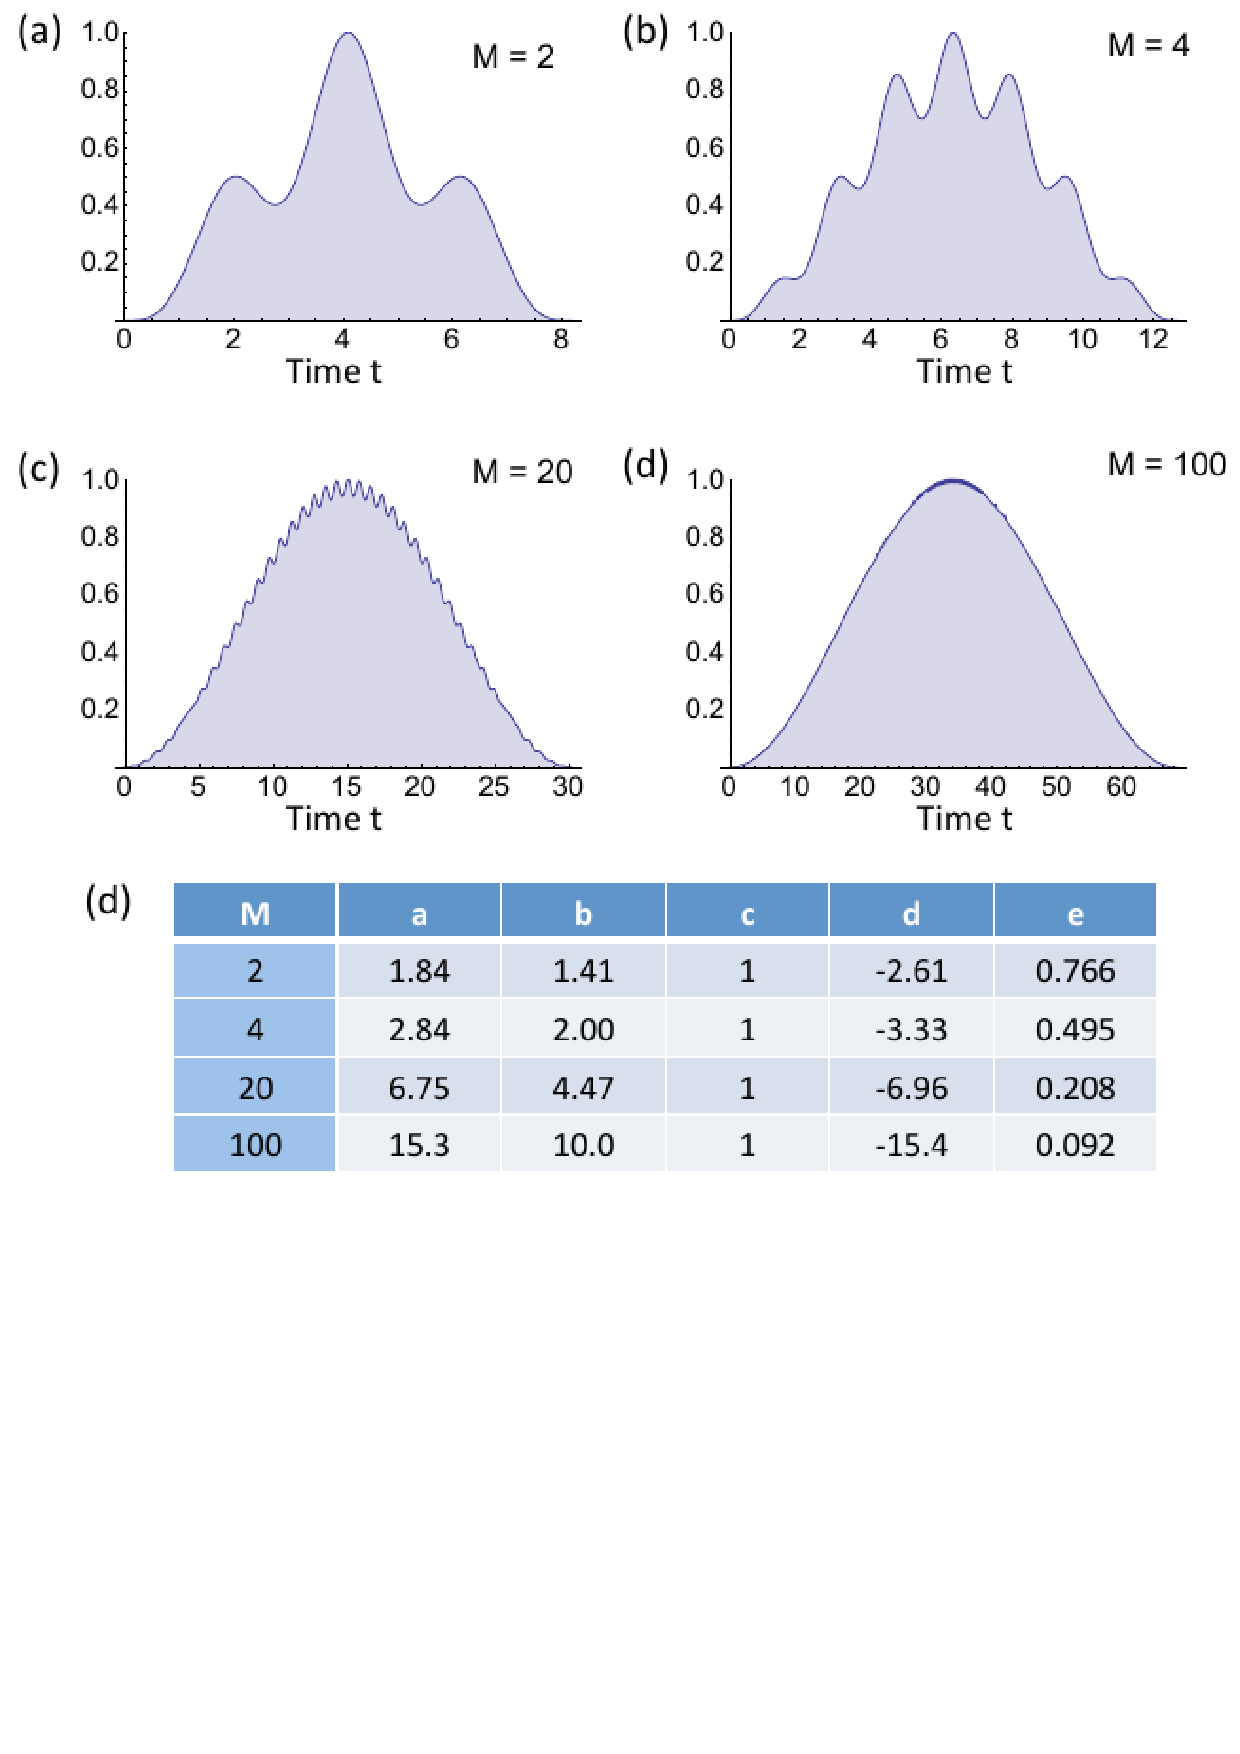
\includegraphics[trim=-50mm 0mm 30mm 0mm, width=0.75\textwidth]{Images/switch_fidelities}
\end{frame}

\subsection{Switch$^2$}
\begin{frame}{Switch$^2$}
	\begin{columns}[T]
		\begin{column}{0.5\textwidth}
			\centering
   			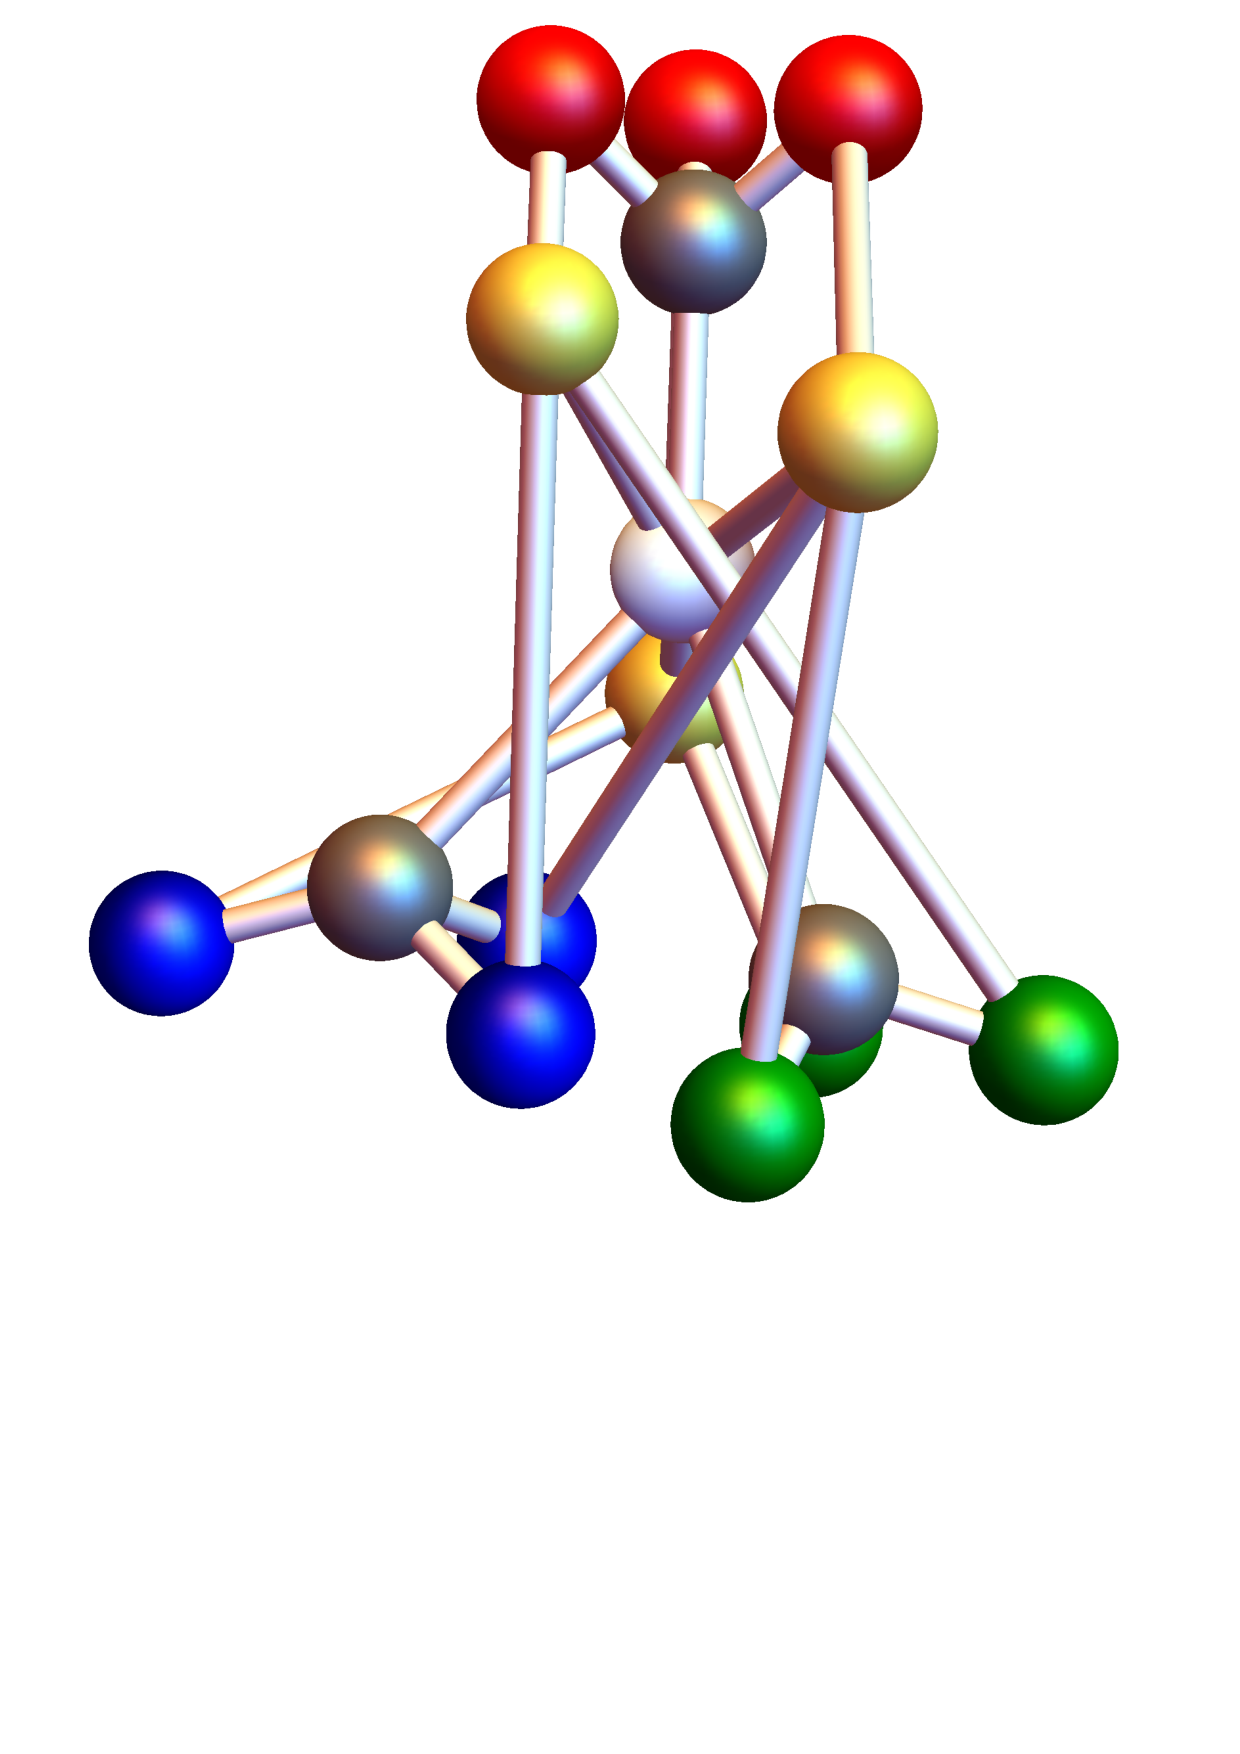
\includegraphics[trim=0mm 0 0 0mm, width=1.2\textwidth]{Images/switch_square}
		\end{column}
		\begin{column}{0.5\textwidth}
			\centering
    		\begin{itemize}
    			\item $h_{u,v} = h_u + h_v \rightarrow $ local potentials are added
    			\item State at vertex $(2,2)$ is transferred to vertex $(3,3)$ or $(4,4)$ at $t = \frac{\pi}{h_2}$
    			\item Symmetry of simple switch $\rightarrow$ transfer from $(2,3)$ to $(3,2)$ or $(2,4)$ to $(4,2)$ with same configuration
    			\item Higher products similar
    		\end{itemize}
		\end{column}
	\end{columns}
%    graph product works with local potentials as well, added at each site, symmetries, more arms.
\end{frame}

\section{Roadmap}
\subsection{Varying Couplings}
\begin{frame}[t]{Varying Couplings}
	\begin{exampleblock}{}
	\setlength\abovedisplayskip{-8pt}
	\begin{center}
		\[H_{XX}=\frac{1}{2}\sum_{i=1}^{N}{J_i\left[\sigma_i^x\sigma_{i+1}^x + \sigma_i^y\sigma_{i+1}^y\right]}\]
	\end{center}
	\end{exampleblock}
	\begin{columns}[T]
		\begin{column}{0.5\textwidth}
			\centering
			Weighted graphs
   			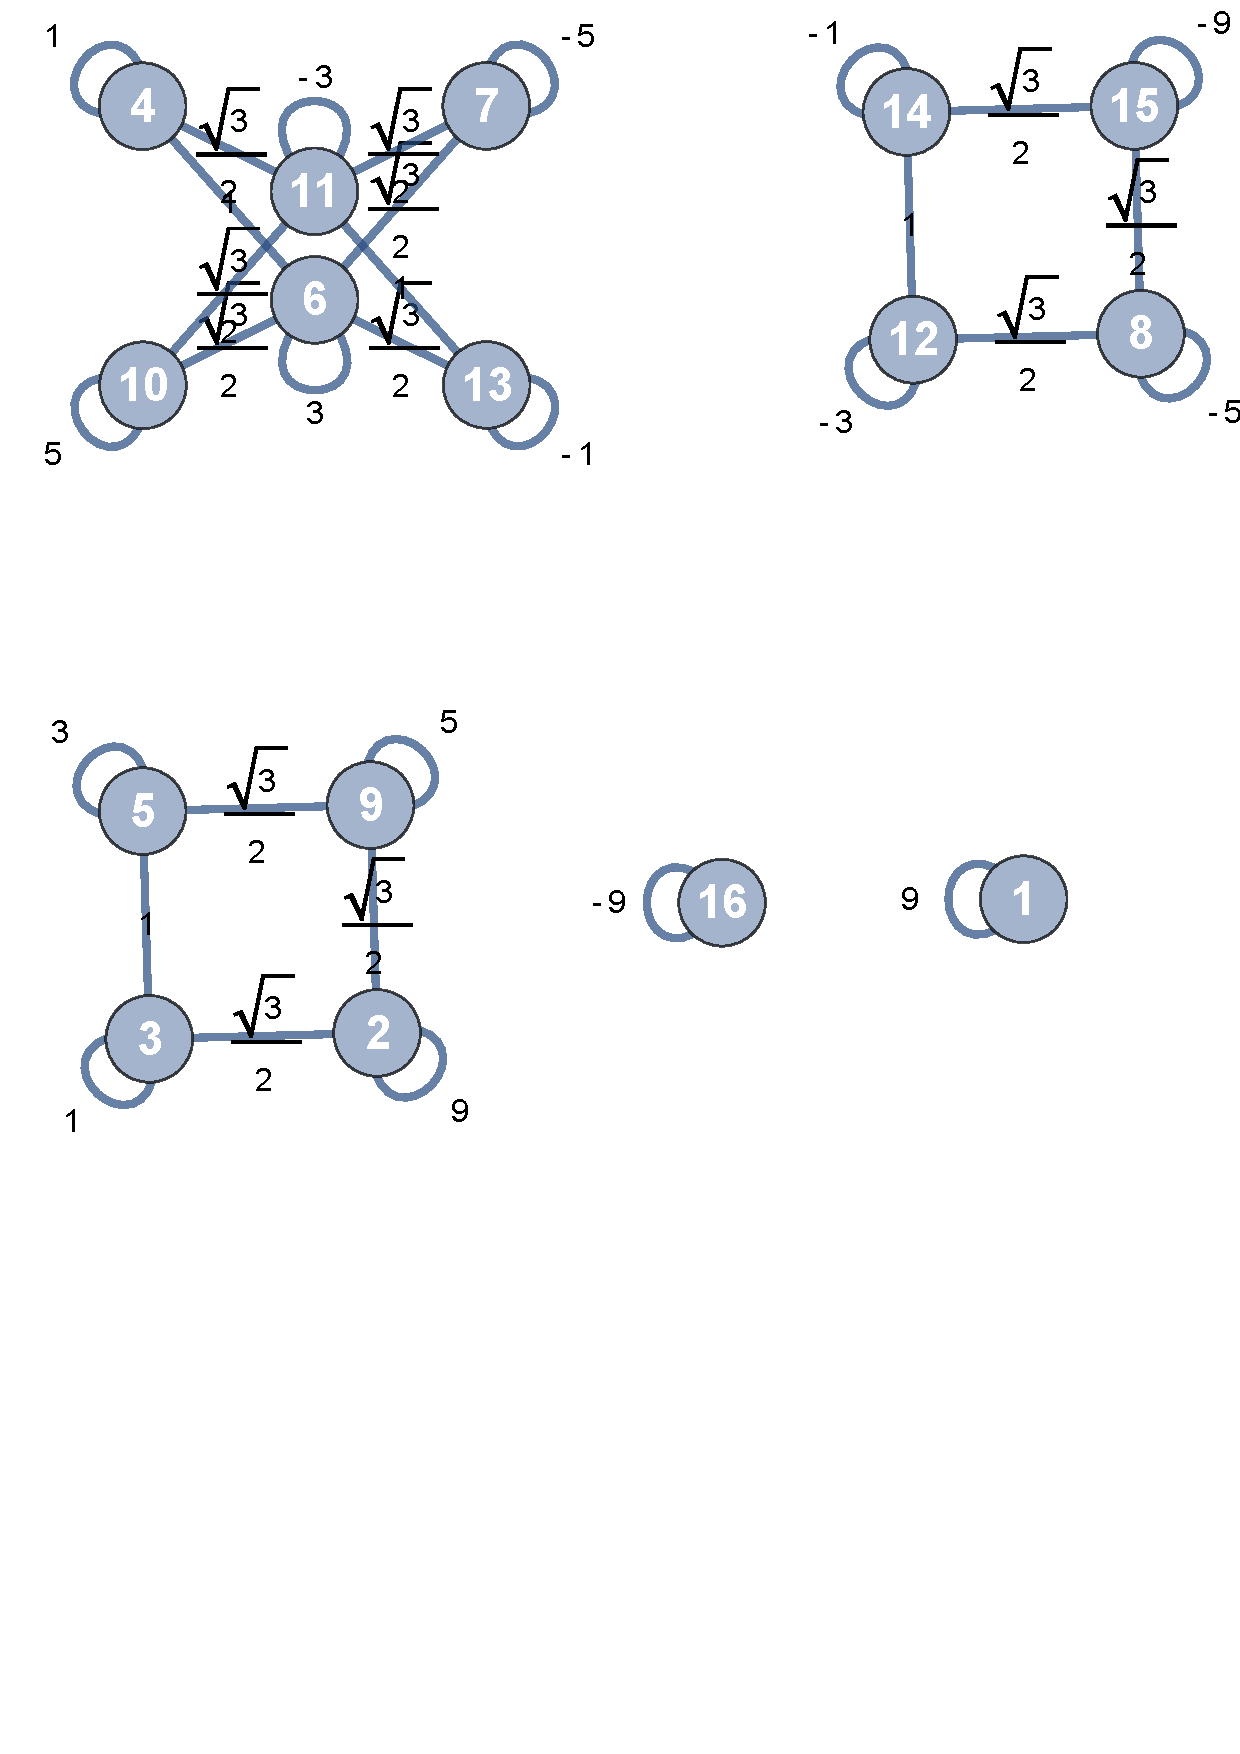
\includegraphics[trim=0mm 0 0 0mm, width=0.8\textwidth]{Images/graph_vary}
		\end{column}
		\begin{column}{0.5\textwidth}
			\centering
			Weighted adjacency matrices
   			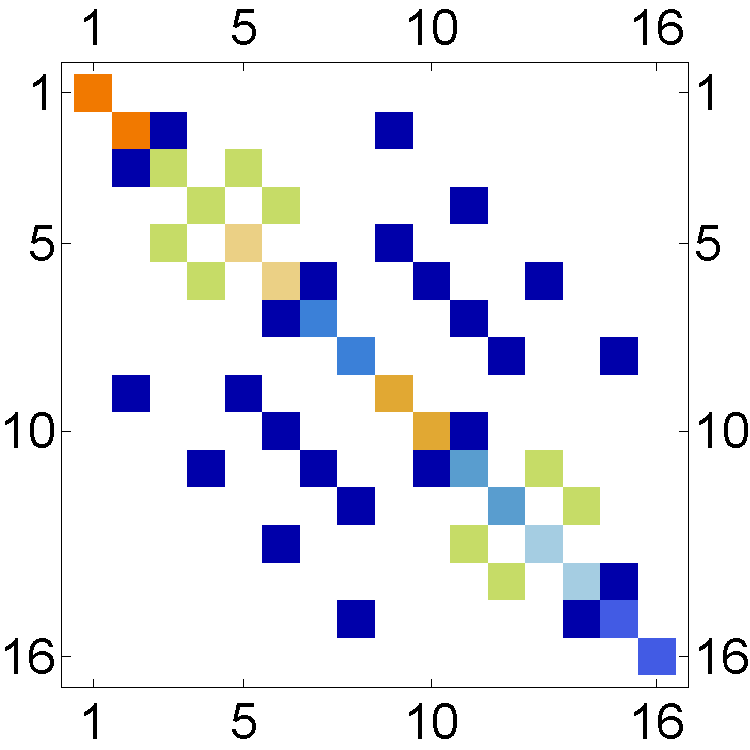
\includegraphics[trim=0mm 0 0 0mm, width=0.7\textwidth]{Images/adj_vary}
		\end{column}
	\end{columns}
	
%    Local couplings leads to much more variety, spin chains with perfect couplings (isomorphism of hilbert spaces to spin n-something particle), not yet looked at switch
\end{frame}

\begin{frame}[t]{Perfect Couplings}
	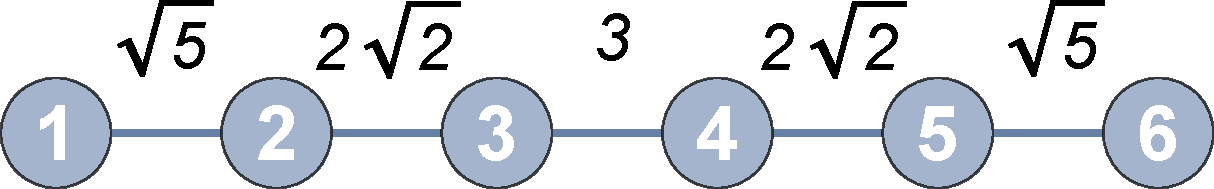
\includegraphics[trim=0mm 0 0 0mm, width=\textwidth]{Images/chain6_perf}
	\begin{itemize}
%		\item Hilbert spaces of same dimensions are isomorphic
		\item Let $J_i = \frac{\lambda}{2}\sqrt{i(N-i)}$
		\item N qubit spin chain with $J_i \leftrightarrow$ Particle with spin $s = \frac{N-1}{2}$ % S_x is angular momentum operator
		\item $H=\lambda S_x \rightarrow U(t)=e^{-\text{i}\lambda t S_x}$
		\item $\braket{N|U(t)|1} = \left( -\text{i}\sin\left(\frac{\lambda t}{2}\right) \right)^{N-1}$
	\end{itemize}	
   	\[H = \begin{pmatrix}
	0 & \sqrt{5} & 0 & 0 & 0 & 0 \\
	\sqrt{5} & 0 & \sqrt{8} & 0 & 0 & 0 \\
	0 & \sqrt{8} & 0 & \sqrt{9} & 0 & 0 \\
	0 & 0 & \sqrt{9} & 0 & \sqrt{8} & 0 \\
	0 & 0 & 0 & \sqrt{8} & 0 & \sqrt{5} \\
	0 & 0 & 0 & 0 & \sqrt{5} & 0 
	\end{pmatrix}\]
%    Local couplings leads to much more variety, spin chains with perfect couplings (isomorphism of hilbert spaces to spin n-something particle), not yet looked at switch also from flattened hypercube
\end{frame}

\subsection{Higher Excitation Subspaces}
\begin{frame}{Higher Excitation Subspaces} %[fragile,t] for listings
	\begin{columns}
		\begin{column}{0.5\textwidth}
			\centering
				\begin{itemize}
		\item PST in larger networks%might be possible for single qubit controlled sites
		\item Control more than one qubit
		\begin{itemize}
			\item Quantum error correction and fault tolerance
		\end{itemize}
		\item Prepare multiple states, send to different target sites
	\end{itemize}
		\end{column}
		\begin{column}{0.5\textwidth}
			\centering
			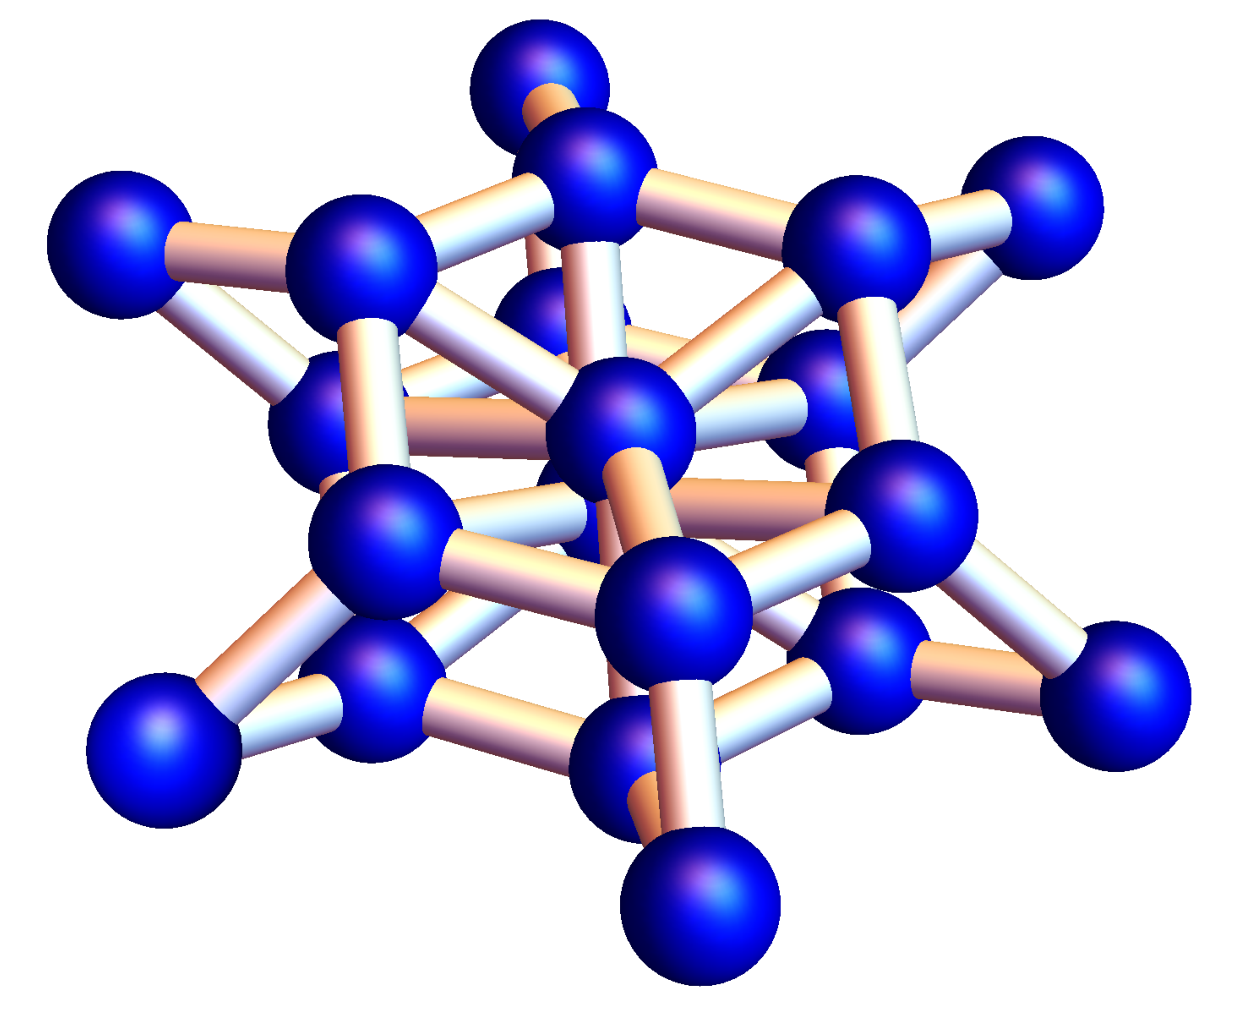
\includegraphics[trim=0mm 0 0 0mm, width=\textwidth]{Images/multispinex}\\
			Calculating higher spin graphs from single spin graphs is an easy task.
		\end{column}
	\end{columns}
	
%	\begin{lstlisting}[language=Python]
%def getEdges(self,spin=1):
%    edges = []
%    for vertex in self.getVertices(spin):
%        dec = self.__decompose(vertex)
%        for comb in combinations(dec,spin-1):
%            neighbours = self.__neighbours([x for x in dec if x not in comb][0])
%            for nn in neighbours:
%                if nn not in comb:
%                    edges += [(vertex,self.__xor(list(comb)+[nn]))]
%        neighbours = []
%    decomposition = []
%    return edges
%	\end{lstlisting}
%    Possibility to control more than one qubit at each site, rings, QEC and fault tolerance, easy to calculate higher spin subspace graphs and hamiltonians, even full hamiltonian
\end{frame}

\subsection{Entanglement}
\begin{frame}{Entanglement}
	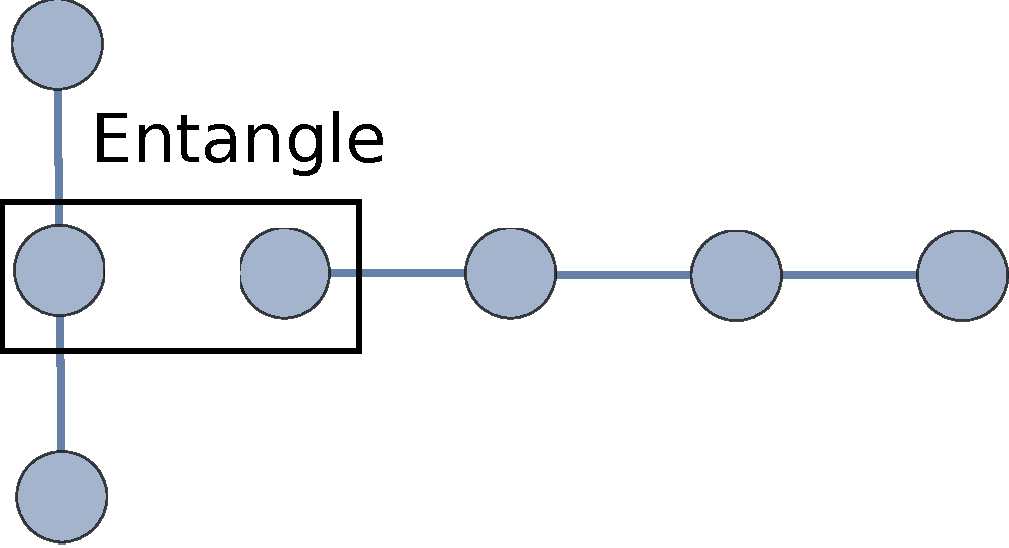
\includegraphics[trim=0mm 0 0 0mm, width=\textwidth]{Images/entanglement}
	\begin{itemize}
		\item 
	\end{itemize}
%    Dynamics of entanglement, teleportation for transport.
\end{frame}

\subsection{Experimental Verification}
\begin{frame}{Experimental Verification}
	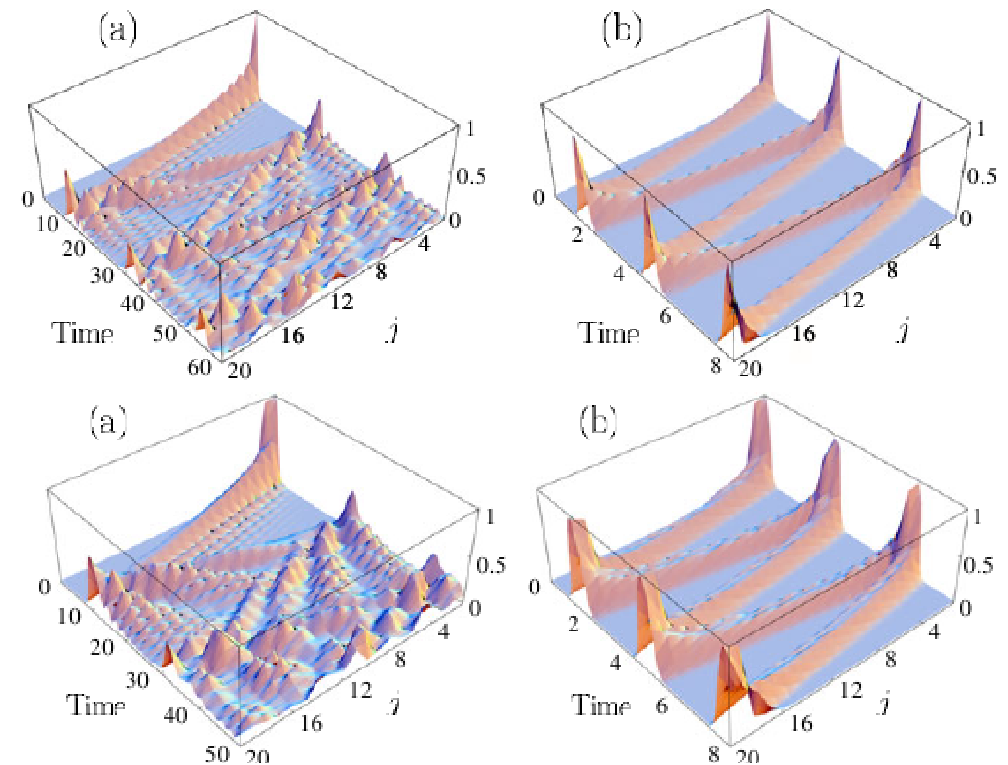
\includegraphics[trim=0mm 0 0 0mm, width=0.9\textwidth]{Images/experiment_chains}
%    Some experiments verify these results, Georgios paper (cm4) for two-spin up subspace analysis and great pictures, quantum dots
\end{frame}

\section{Goal}
\begin{frame}{Goal}
	\begin{itemize}
		\item Framework for engineering spin chains with given properties
		\item Define certain constraints for hamiltonian
		\item Single spin subgraph should yield a network capable of PST
	\end{itemize}
%    Define general constraints on hamiltonians so that the single spin subspace graph leads to a network automatically capable of perfect state transfer, hints: symmetry, EV difference quotient rational, connectivity.
\end{frame}

\end{document}
